% \documentclass[a4paper,10pt]{article}
% \usepackage[utf8]{inputenc}
% \usepackage{fullpage}
% \usepackage{graphicx} % pour insérer des images
% \usepackage{epstopdf}
% % Les N, Z..., math quoi
% \usepackage{amsthm}
% \usepackage{amsmath}
% \usepackage{stmaryrd}
% \usepackage{amsfonts}
% \usepackage{tikz}
% \usepackage{tikz-qtree}
% % les figure imbriquées
% \usepackage{epsfig}
% \usepackage{subfigure}
% \usepackage[francais]{babel}
% \usepackage[algoruled,french,onelanguage]{algorithm2e}


% %opening
% \title{}
\todo[inline]{Perfs + FP/FN}
\todo[inline]{Limitations : obfuscation du CFG}

\section{Comparaison de graphes de flots de contrôles et détection}
On cherche à identifier des parties d'un graphe de flot inconnu qui seraient présentes dans une collection de graphes de flots de contrôles donnée (base de malware par exemple).
On note T le graphe de flot de test à analyser.
\\
On définit formellement la reconnaissance de deux parties communes dans deux graphes par l'existence d'un isomorphisme de sous-graphe entre un graphe de la base et T.
\begin{defi}\label{def-graphe-oriente}
Un graphe orienté et étiqueté $T=(V, L, l, E)$ est composé par les ensembles finis V, L, E, et la fonction totale $l:V\rightarrow L$.
V est l'ensemble des sommets de T, L un ensemble d'étiquettes, l la fonction donnant l'étiquette d'un sommet, et $E\subset V\times V$ est l'ensemble des arcs de T tel que $(t, h)\in E$ ssi il y a un arc entre le sommet t et le sommet h.
\end{defi}

\begin{defi}\label{def:valence}
 La valence d'un sommet d'un graphe est le nombre de fils de ce sommet.
\end{defi}

Les graphes sur lesquels nous sommes amenés à travailler peuvent être partiels : il y a des branches qui peuvent être inconnues. De plus pour simplifier les algorithmes impliqués dans la recherche de parties communes à plusieurs graphes, il est pratique de forcer les fils de chaque sommet à être ordonnés.

\begin{defi}\label{def:gf}
Un graphe de flot est un graphe orienté et étiqueté vérifiant :
\begin{enumerate}
%  \item Chaque sommet a une étiquette, et
%  \begin{enumerate}
%   \item La valence d'un sommet est son nombre de fils
\item On associe à chaque étiquette une arité dans $\mathbb{N}$ : il s'agit de la valence maximale pour tous les sommets ayant cette étiquette, et
%   \item L'arité associée à une étiquette est la valence maximale pour les sommets ayant cette étiquette, et
%  \end{enumerate}
 \begin{enumerate}
  \item Si la valence de chaque sommet est égale à l'arité de son étiquette, le graphe de flot est dit complet
  \item Dans le cas contraire, il s'agit d'un graphe de flot incomplet
 \end{enumerate}
 \item Les fils de chaque sommet sont ordonnés : les arcs ont pour label l'ordre i du fils (où i est un entier compris entre 1 et la valence du sommet)\\
       L'ensemble des arcs est $E\subset V\times \mathbb{N}\times V$ tel que $(t, i, h)\in E$ ssi il y a un arc numeroté i entre le sommet t et le sommet h.
%  \item La valence de ses sommets est bornée
\end{enumerate}
\end{defi}
% Un graphe de flot (définition \ref{def:gf}) est un graphe orienté particulier.

% Le point 1 force à expliciter les fils ; par exemple un \emph{JCC} a nécessairement deux successeurs, selon que la condition vérifiée est satisfaite ou non. Les sites incomplets sont une extension autorisant que certains fils ne soit pas connus (on peut les omettre dans la représentation ou ajouter un fils artificiel $\bot$).
% Le point 2 est une restriction forte utilisée pour rendre la détection possible en un temps raisonnable.

\section{Isomorphisme de graphes et de sous-graphes de flot}


Deux graphes de flot sont isomorphes s'ils vérifient les
propriétés de la définition \ref{def-iso-go}. On définit le sous-graphe d'un graphe T selon la définition \ref{def-sousgrapheflot}.
% il est
% important de noter qu'un sous-graphe a des sommets pris arbitrairement au graphe de base mais que ses arcs sont exactement tous ceux
% du graphe de base qui s'appliquent aux sommets choisis. 
Notre problème
consiste donc, à partir du graphe de flot T à analyser, à déterminer si un de ses sous-graphes est isomorphe à un des graphes de flot de la base.
Par exemple sur la figure \ref{fig:ex-gf-sous-gf}, on cherche à savoir si le graphe P peut-être vu comme identique à un sous-graphe de T en préservant sa
structure. Ici le graphe P est isomorphe au sous-graphe constitué des sommets $\{d, e, a\}$ comme à celui formé par les sommets $\{b, d, a\}$.


\begin{figure}[ht]
\begin{center}
  \subfigure[Graphe de flot T]{
\label{fig:ex-gf}
% \epsfig{figure=images/def-graphe2.pdf,height=3.5cm}}\quad
\epsfig{figure=supports/algos/images/c_gTGF.pdf,height=3.5cm}}\quad
  \subfigure[Graphe de flot P, isomorphe à un sous-graphe de T]{
\label{fig:ex-sous-gf}
% \epsfig{figure=images/def-graphe1.pdf,height=3cm}}\\
\epsfig{figure=supports/algos/images/c_gPGF.pdf,height=3cm}}\\
\end{center}
\caption{Exemple de graphe de flot et d'un sous-graphe}
\label{fig:ex-gf-sous-gf}
\end{figure}

\begin{defi}\label{def-iso-go}
Soit $T=(V_T, L_T, l_T, E_T)$ et $P=(V_P, L_P, l_P, E_P)$ deux graphes de flot. Ils sont dits isomorphes s'il existe une bijection $f:V_T\rightarrow V_P$ entre les sommets de T et ceux de P et
si f préserve la structure d'adjacence des graphes avec l'ordre des fils, c'est à dire si \\
$\forall u, v \in V_T$ et $i\in\mathbb{N} : (u, i, v) \in E_T \Leftrightarrow (f(u), i, f(v)) \in E_P$.
\end{defi}

% \begin{defi}\label{def-sousgraphe}
% Un graphe orienté $P=(V_P, E_P)$ est un sous-graphe du graphe $T=(V_T, E_T)$ si et seulement si $V_P \subset V_T$, et $E_P=\{(t, h)\in E_T / t, h \in V_P \}$
% \end{defi}

\begin{defi}\label{def-sousgrapheflot}
Un graphe de flot $P=(V_P, L_P, l_P, E_P)$ est un sous-graphe du graphe de flot $T=(V_T, L_T, l_T, E_T)$ si et seulement si $V_P \subset V_T$, $E_P\subset\{(t, i, h)\in E_T / t, h \in V_P \}$, et $\forall u\in V_P, l_P(u)=l_T(u)$
\end{defi}

\begin{defi}\label{def-sousgrapheflot-induit}
Le sous-graphe induit d'un graphe de flot $T=(V_T, L_T, l_T, E_T)$ à partir de l'ensemble de sommets $V_P \subset V_T$ est le graphe de flot $P=(V_P, L_P, l_P, E_P)$ tel que $E_P=\{(t, i, h)\in E_T / t, h \in V_P \}$, $L_P=L_T$, et $l_P=l_{T\vert V_P}$.
\end{defi}


% TODO: def \ref{def-sousgraphe} et def \ref{def-sousgraphe2} sont équivalentes pour les sites!

\section{Sites}
En pratique on va choisir un certain nombre de sous-graphes particuliers de la base, appelés sites, qui seront les motifs qu'on cherche à détecter : on note généralement P un graphe de motif. Un site est un graphe de flot ayant une racine (définition \ref{def-site}). Un site peut être un sous-graphe d'un graphe de flot (définition \ref{def-soussite}) comme dans l'exemple de la figure \ref{fig:ex-gf-site}.

\begin{defi}\label{def-site}
Un site P est un graphe de flot ayant une racine : un sommet à partir duquel on peut atteindre n'importe quel autre sommet de P
\end{defi}

\begin{defi}\label{def-soussite}
On appelle sous-site d'un graphe de flot $T$ tout site étant un sous-graphe de $T$.
\end{defi}

\begin{figure}[ht]
\begin{center}
  \subfigure[Graphe de flot T]{
\label{fig:ex-gf}
% \epsfig{figure=images/def-graphe2.pdf,height=3.5cm}}\quad
\epsfig{figure=supports/algos/images/c_gTGF.pdf,height=3.5cm}}\quad
  \subfigure[Site P, de racine b, isomorphe à un sous-graphe de T]{
\label{fig:ex-site}
% \epsfig{figure=images/def-graphe1.pdf,height=3cm}}\\
\epsfig{figure=supports/algos/images/c_gPsite.pdf,height=3cm}}\\
\end{center}
\caption{Exemple de graphe de flot et d'un sous-site}
\label{fig:ex-gf-site}
\end{figure}


% \begin{defi}\label{def-site-incomplet}
% Un site incomplet est un site dans lequel certains n\oe uds n'ont pas le bon nombre de fils mais ces fils sont tout de même ordonnés.
% \end{defi}

\section{Problème de la détection des sites isomorphes}
Le problème se pose alors de la manière suivante. On dispose d'une liste de sites et %provenant de multiples graphes de flot de contrôle différents.
on veut déterminer, dans le graphe de flot T, les sites qui sont isomorphes à (au moins) un site présent dans la liste connue. Dans une optique de détection, il est aussi nécessaire d'associer chaque site de la base connue au programme dont il est issu.

On a alors trois problèmes successifs, de difficulté croissante et faisant intervenir différents algorithmes.
\begin{pb}\label{pbisog}
 Comment savoir si deux graphes sont isomorphes ?
\end{pb}

\begin{pb}\label{pbisosg}
 À partir d'un site $P$ et d'un graphe de flot $T$, comment savoir si $P$ est un sous-site de $T$ ?
\end{pb}

% Dans le problème~\ref{pbisosg}, on nomme $P$ le site de motif et $T$ le graphe de test.

\begin{pb}\label{pbisosgbase}
 À partir d'un ensemble de sites $L_P$ et d'un graphe de flot $T$, comment savoir s'il existe $P\in L_P$ tel que $P$ est un sous-site $T$ ?
\end{pb}

\section{Représentation sous forme matricielle}
\begin{figure}[ht]
\begin{center}
  \subfigure[Graphe T]{
\label{fig:ex-graphe}
% \epsfig{figure=images/def-graphe2.pdf,height=3.5cm}}\quad
\epsfig{figure=supports/algos/images/c_gT.pdf,height=3.5cm}}\quad
  \subfigure[Graphe P, isomorphe à un sous-graphe de T]{
\label{fig:ex-sg}
% \epsfig{figure=images/def-graphe1.pdf,height=3cm}}\\
\epsfig{figure=supports/algos/images/c_gP.pdf,height=3cm}}\\
\end{center}
\caption{Exemple de graphe et d'un sous-graphe}
\label{fig:ex-graphe-sg}
\end{figure}

Dans cette section et la suivante, on traite le cas général de l'isomorphisme de graphes et de sous-graphes orientés comme dans l'exemple de la figure \ref{fig:ex-graphe-sg}. En particulier ces graphes ne sont, sauf mention du contraire, pas étiquetés et les fils des sommets ne sont pas ordonnés. Nous redonnons les définitions précédentes de graphes orientés, de sous-graphe et sous-graphe induit ainsi que d'isomorphisme de graphes dans le cas des graphes orientés quelconques.

\begin{defi}\label{def-graphe}
Un graphe orienté $T=(V, E)$ est composé par les ensembles finis V et E.
V est l'ensemble des sommets de T, $E\subset V\times V$ est l'ensemble des arcs de T tel que $(t, h)\in E$ ssi il y a un arc entre le sommet t et le sommet h.
\end{defi}

\begin{defi}\label{def-sousgraphe}
Un graphe orienté $P=(V_P, E_P)$ est un sous-graphe du graphe orienté et étiqueté $T=(V_T, E_T)$ si et seulement si $V_P \subset V_T$ et $E_P\subset\{(t, h)\in E_T / t, h \in V_P \}$.
\end{defi}

\begin{defi}\label{def-sousgraphe-induit}
Le sous-graphe induit d'un graphe orienté et étiqueté $T=(V_T, E_T)$ à partir de l'ensemble de sommets $V_P \subset V_T$ est le graphe $P=(V_P, E_P)$ tel que $E_P=\{(t, h)\in E_T / t, h \in V_P \}$.
\end{defi}

\begin{defi}\label{def:isog}
Soit $T=(V_T, E_T)$ et $P=(V_P, E_P)$ deux graphes orientés. Ils sont dits isomorphes s'il existe une bijection $f:V_T\rightarrow V_P$ entre les sommets de T et ceux de P et si f préserve la structure d'adjacence des graphes, c'est à dire si : $\forall u, v \in V_T, (u, v) \in E_T \Leftrightarrow (f(u), f(v)) \in E_P$.
\end{defi}

On peut représenter les graphes sous forme de matrices. On définit la matrice d'adjacence M d'un graphe T suivant les arcs qu'il contient si ses sommets sont ordonnés dans $V=\{v_1, v_2, ..., v_n\}$. Ensuite s'il y a un arc du sommet $v_i$ vers le sommet
$v_j~\mbox{alors}~M_{i, j}=~1,~\mbox{sinon}~M_{i,~j}=~0$ (définition \ref{def-adjmatrice}).
Pour un graphe donné dont les sommets ne sont pas ordonnés, on peut choisir arbitrairement un ordre à ses sommets et dans ce cas il y a autant de matrices d'adjacence possibles pour ce graphe qu'il y a de permutations de ses sommets. 

Par la suite la matrice $M_T$ d'adjacence d'un graphe T représente une de ces matrices, arbitrairement fixée à la première occurence de $M_T$.
En théorie le choix d'une matrice d'adjacence n'a pas d'impact sur les solutions trouvées puisque toutes les matrices d'adjacence d'un graphe sont les mêmes à une permutation des sommets près, et que par la suite on n'utilise des égalités entre ces matrices qu'à une permutation près.
Dans les implémentations il est facile de fixer arbitrairement un ordre aux sommets. 
% En mémoire chaque sommet du graphe est réprésenté par une structure, il suffit de les ordonner selon l'adresse mémoire de cette structure. Enregistrés dans un fichier, les sommets sont décrits un par un, ce qui donne un ordre naturel.

\begin{defi}\label{def-adjmatrice}
Soit T=(V, E) un graphe orienté à $n \in \mathbb{N}$ sommets ordonnés. La matrice d'adjacence M associée à T est la matrice $n \times n$ définie par : 
$M_{i, j} = \left\{
  \begin{array}{ll}
	  1 & si\ (i, j) \in E
	\\0 & \mbox{sinon.}
  \end{array}
\right.
$
\end{defi}

Par exemple, les graphe P et T de la figure \ref{fig:ex-graphe-sg} ont pour matrice d'adjacence les matrices de la figure~\ref{fig:mat-adj}. 

% \begin{figure}[ht]
% \begin{center}
% $M_{i, j} = \begin{array}{r|ccc}  & a & b & c \\ \hline a & 0 & 1 & 1 \\ b & 0 & 0 & 1 \\ c & 0 & 0 & 0 \end{array}$
% \\
% \end{center}
% \caption{Matrice d'adjacence du graphe P}
% \label{fig:mat-adj}
% \end{figure}

\begin{figure}[ht]
\begin{center}
  \subfigure[$M_T$]{
\label{fig:mat-adjT}
$M_{i, j} = \begin{array}{r|ccccc}  & a & b & c & d & e \\ \hline a & 0 & 0 & 0 & 0 & 0 
							\\ b & 1 & 0 & 0 & 1 & 0
							\\ c & 0 & 0 & 0 & 0 & 0
							\\ d & 1 & 0 & 0 & 0 & 1
							\\ e & 1 & 0 & 1 & 0 & 0
 \end{array}$}\quad
  \subfigure[$M_P$]{
\label{fig:mat-adjP}
$M_{i, j} = \begin{array}{r|ccc}  & a & b & c \\ \hline a & 0 & 0 & 0 \\ b & 1 & 0 & 1 \\ c & 1 & 0 & 0 \end{array}$}\\
\end{center}
\caption{Matrices d'adjacence des graphes T et P}
\label{fig:mat-adj}
\end{figure}

Le problème de l'isomorphisme peut alors se reformuler. Deux graphes T et P sont isomorphes si et seulement si il existe une permutation $\sigma$ des sommets du graphe T telle
que $M_{\sigma(T)}=M_P$. Il est donc nécessaire et suffisant qu'il existe une matrice de permutation K telle que $M_P = K.M_T.K^t$ (car $K^{-1}=K^t$ pour une matrice de permutation).


On note $n_T$ et $n_P$ le nombre de sommets des graphes T et P, respectivement. Pour l'isomorphisme de sous-graphe on cherche un sous-ensemble $\{s_1, s_2, ..., s_{n_P}\}$ de $n_P$ sommets de T et un sous-ensemble d'arcs de T entre les sommets $\{s_1, s_2, ..., s_{n_P}\}$ tels que le sous-graphe défini par ces sommets et ces arcs soit isomorphe à P. Supposons qu'il existe un tel isomorphisme et on note $\sigma$ de $\mathfrak{S}(n_T)$ telle que $\forall i \leq n_P,\ \sigma(s_i) \leq n_P$ donnant les $n_P$ sommets de T y participant. Les autres éléments n'ont pas d'importance
puisqu'ils ne participent pas à l'isomorphisme recherché. Soit K la matrice de permutation associée à $\sigma$.
Les arcs présents dans P doivent être présents dans le sous-graphe de T induit à partir de $\{s_1, s_2, ..., s_{n_P}\}$, ce qui en terme de matrices d'adjacence équivaut à ce que, si on note la matrice du graphe induit $M_{\sigma(T)}=K.M_T.K^t$, ses éléments, pour les sommets qui participent à l'isomorphisme (les $n_P$ premiers sommets), soient supérieurs aux éléments à la même place dans $M_P$ : $\forall k,l\leq n_P, (M_P)_{k,l}\leq (K.M_T.K^t)_{k,l}$. Il suffit alors de réduire la taille de la matrice en utilisant une matrice $I_{n_P, n_T}$ définie par
$(I_{n_P, n_T})_{i, j} = \left\{
  \begin{array}{ll}
	  1 & si\ i=j
	\\0 & \mbox{sinon}
  \end{array}
\right.
$.


Dans ce cas, et si on pose $Q=I_{n_P, n_T}.K$ avec $Q\in \mathbb{M}_{n_P, n_T}$, on a $Q.M_T.Q^t=I_{n_P, n_T}.K.M_T.K^t.I_{n_T, n_P}$, les deux matrices $M_P$ et la condition devient : il est nécessaire qu'il existe une matrice $Q\in \mathbb{M}_{n_P, n_T}$ telle que pour toute ligne k et colonne l de $M_P$, $(M_P)_{k,l}\leq (Q.M_T.Q^t)_{k,l}$.

Inversement, s'il existe une matrice de permutation $K$ (carrée de taille $n_T$) telle que, en notant $Q=I_{n_P, n_T}.K$, $\forall k,l\leq n_P, (M_P)_{k,l}\leq (Q.M_T.Q^t)_{k,l}$ alors il existe bien un isomorphisme de graphes entre un sous-graphe de T et P.

Dans l'exemple des graphes de la figure \ref{fig:ex-graphe-sg}, P est isomorphe au sous-graphe de T composé des sommets $\{d, e, a\}$ en faisant correspondre les couples (a, a), (d, b) et (e, c) entre T et P, soit la
permutation $\sigma$ telle que $\sigma(1)=~1,\ \sigma(4)=~2\ et\ \sigma(5)=~3$. La matrice de permutation K est donnée en figure \ref{fig:mat-perm}.
La transformation qu'elle induit est donnée par la matrice $M_{\sigma(T)}$ en figure \ref{fig:mat-Tsigma}. Il paraît alors évident qu'en ne prenant que la sous-matrice $3\times 3$, on obtient $M_P$, opération
réalisée à l'aide de $I_{n_P, n_T}$ (figure \ref{fig:mat-Inm}).


\begin{figure}[ht]
\begin{center}
  \subfigure[Matrice de permutation K]{
\label{fig:mat-perm}
$\left( \begin{array}{ccccc}
1 & 0 & 0 & 0 & 0 \\
0 & 0 & 0 & 1 & 0 \\
0 & 0 & 0 & 0 & 1 \\
0 & 1 & 0 & 0 & 0 \\
0 & 0 & 1 & 0 & 0 \end{array} \right)$
}\quad
  \subfigure[$M_{\sigma(T)}=K.M_T.K^t$]{
\label{fig:mat-Tsigma}
$\left( \begin{array}{ccccc}
0 & 0 & 0 & 0 & 0 \\
1 & 0 & 1 & 0 & 0 \\
1 & 0 & 0 & 0 & 1 \\
1 & 1 & 0 & 0 & 0 \\
0 & 0 & 0 & 0 & 0 \end{array} \right)$
}\quad
\subfigure[$I_{n_P, n_T}$]{
\label{fig:mat-Inm}
$\left( \begin{array}{ccccc}
1 & 0 & 0 & 0 & 0 \\
0 & 1 & 0 & 0 & 0 \\
0 & 0 & 1 & 0 & 0 \end{array} \right)$
}\\
\end{center}
\caption{Matrices pour la démonstration sur l'exemple de T et P}
\label{fig:mat-exemplesub}
\end{figure}



%$I^{n, m}_{i, j}=1$ si $i=j$, $I^{n, m}_{i, j}=0$ 


L'approche par force brute demande de parcourir toutes les matrice de permutations de taille $n_T$ : il y en a $n_P!$. Pour chaque matrice de permutation, une matrice transposée est déterminée et plusieurs multiplications matricielles sont faites sur des matrices de taille $n_T.n_T$, opération réalisable au pire en $n_T^3$. La complexité de cette approche dans le pire des cas est donc $O(n_T^3.n_T!)$.


\section{Algorithme d'Ullmann}
L'algorithme d'Ullmann est le plus connu pour résoudre le problème \ref{pbisosg} d'isomorphisme de sous-graphes \cite{Ull76} dans le cas général des graphes orientés. Il s'applique à un graphe de motif P à détecter et à un graphe T dans lequel faire la reconnaissance. Comme détaillé par la suite, sa complexité est exponentielle en le nombre de sommets maximal du graphe de motif P.


De plus, si on veut l'utiliser pour résoudre le problème \ref{pbisosgbase} de recherche d'isomorphismes de sous-graphes dans une base de graphes de motifs, il est nécessaire de l'appliquer pour chaque graphe dans la base, la complexité est alors linéaire en le nombre de graphes dans la base.\\

Puisqu'il est complet pour le problème d'isomorphisme de sous-graphes, ce sera l'algorithme de référence auquel on pourra comparer les heuristiques sur le plan de la complétude, de la complexité, et du temps d'exécution.\\

Nous présenterons d'abord l'algorithme d'Ullmann dans le cas de graphes orientés quelconques puis nous y ferons des restrictions pour l'adapter au cas des graphes de flot.
\subsection{L'algorithme d'Ullmann pour l'isomorphisme de sous-graphes}
L'algorithme d'Ullmann repose
sur le concept de retour sur traces (ou \emph{backtracking}) pour trouver successivement tous les sous-graphes isomorphes au 
graphe de motif. Cette approche a ensuite été largement améliorée par Ullmann à l'aide de l'utilisation d'une technique de
vérification à priori permettant d'éliminer de nombreux candidats sans avoir à les tester entièrement.

\subsubsection{Backtracking simple}
Soit $T=(V_T, E_T)$ un graphe et $P=(V_P, E_P)$ un graphe dont on cherche à connaître les sous-graphes de T avec lesquels il est isomorphe.
On note $n_T=Card(V_T)$ et $n_P=Card(V_P)$ les nombres de n\oe uds de chaque graphe.
L'idée consiste à partir d'un sommet de P, à l'associer à un sommet de T, de vérifier si l'association créée est bien un
isomorphisme de sous-graphe. Si c'est le cas, on prend un autre sommet de P à associer avec un sommet de T pas encore
inclus dans la transformation. Si ce n'est pas un isomorphisme de sous-graphe, on retire la dernière association faite, et on
repart en incluant un autre sommet. Et ainsi de suite. Lorsqu'on a une transformation utilisant tous les sommets de P et définissant
un isomorphisme avec un sous-graphe de T, on la met de coté (c'est une solution), et on revient en arrière pour trouver les autres
solutions.


La manière de tester si on a bien obtenu un isomorphisme est celle décrite précédemment à l'aide de la représentation matricielle.
On définit la matrice de permutation K de la transformation,
puis la matrice $I_{n_P, n_T}$ permettant le redimensionnement d'une matrice, et on regarde si la relation $\forall k,l\leq n_P, (M_P)_{k,l}\leq (I_{n_P, n_T}.K.M_T.K^t.I_{n_T, n_P})_{k,l}$ est
vérifiée.
\\

La première remarque à faire sur le principe donne la validité de cet algorithme. Si deux graphes sont isomorphes et ont au moins 2 sommets,
alors il existe deux sous-graphes respectifs de chacun des graphes, avec un sommet de moins, tels que les deux sous-graphes sont isomorphes.
De ce fait, en augmentant progressivement la taille de chaque sous-graphe de P donnant un isomorphisme, on atteint tous les sous-graphes isomorphes à T.


Une deuxième remarque peut être faite : on peut dès le départ savoir que certaines associations ne donneront pas lieu à un sous-graphe. Avec les graphes P et T
de la figure \ref{fig:ex-graphe-sg}, il est clair que le sommet c du graphe P ne peut pas être associé au sommet c du graphe T. En effet $c_P$ a stricement plus d'arcs
entrant que $c_T$, la structure autour de $c_P$ ne pourrait donc pas être préservée par un isomorphisme. On construit une matrice $C^0 \in \mathbb{M}_{n_P, n_T}$ telle que, pour
$i\le n_P, j\le n_T$, on n'essaie d'associer les sommets i et j que si $C^0_{i, j}=1$. En prenant en compte la remarque précédente, on définit alors
\\

$C^0_{i, j} = \left\{
  \begin{array}{ll}
	  1 & \mbox{si le nombre d'arcs entrant est plus grand pour i dans P que pour j dans T,} \\
	    &  \mbox{et si le nombre d'arcs sortant est plus grand pour i dans P que pour j dans T}
	\\0 & \mbox{sinon.}
  \end{array}
\right.
$
\\
Les conditions sur les inégalités sont prises au sens large.
\\

Le calcul effectif du nombre d'arcs entrant (respectivement sortant) d'un sommet d'un graphe se fait simplement à partir de sa matrice d'adjacence en
additionnant, à colonne (respectivement ligne) constante correspondant au sommet, les valeurs de la matrice sur toutes les lignes (respectivement colonnes).
\\

L'algorithme est détaillé dans la figure \ref{algo:ullman} : il consiste à associer chaque sommet de P à un sommet de T. On note i le numéro du prochain sommet de P à associer à un sommet de T. On démarre donc avec i=1.
On conserve la permutation $\sigma$ sous la forme d'un ensemble F d'éléments de couples de la forme $(i, j)$ avec $i\in T$, et $j\in P$. La première étape
consiste donc à initialiser les matrices que l'on va utiliser ($M_T,\ M_P,\ I_{n_P, n_T},\ et\ C^0$). Une fois l'initialisation faite, pour parcourir toutes les possibilités, on
utilise la procédure \emph{backtrack} en partant d'une matrice de possibilités $C^0$, de i=1, et d'un ensemble F vide. 
% Cette procédure commence par vérifier si la
% situation courante est une solution d'isomorphisme de sous-graphe. Pour cela il faut d'une part que le sous-graphe soit de la taille de P, et d'autre part que ce soit bien un isomorphisme
% avec P, c'est à dire que $M_P=I_{n_P, n_T}^t.K.M_T.K^t.I_{n_P, n_T}$ soit vérifiée. Si la situation courante est une solution, on arrête l'algorithme et on renvoie la solution. Si ce n'était pas
% une solution, p
Pour chaque association possible de i dans T avec un élément j de P (possibilité inscrite dans $C^0$), on ajoute $(i, j)$ à F, on met à jour C (les associations choisies ne pourront
plus l'être ensuite), on détermine les matrices d'adjacence des sous-graphes induits de T et P par les associations choisies dans F, notées $S_T$ et $S_P$ respectivement, ainsi que la matrice de permutation K définie par F.
% et on appelle \emph{backtrack} avec la matrice C, l'entier i+1, et F mis à jour dans le cas où l'élément ajouté donne toujours un isomorphisme entre les sous-graphes
% $S_T$ et $S_P$ considérés par ajouts successifs. 
On peut alors vérifier qu'il y a un isomorphisme de sous-graphe entre les graphes induits de P et T avec la relation suivante : $\forall k,l\leq i, (S_P)_{k,l}\leq (K.S_T.K^t)_{k,l}$, détaillée dans la section précédente.
\begin{itemize}
 \item Si c'est le cas et que $i=n_P$ alors on a trouvé un isomorphisme de sous-graphe entre P et T, on le renvoie puis.
 \item Si c'est le cas mais que $i\ne n_P$ alors on continue à chercher à ajouter des éléments à l'isomorphisme en appelant \emph{backtrack} avec $C'$, $i+1$ et F.
 \item Si ce n'est pas le cas, on ne fait rien.
\end{itemize}
Ensuite il suffit de retirer la dernière association $(i, j)$ et de tester l'association suivante. 

Il est à noter qu'on peut déterminer la matrice de permutation K à partir de l'ensemble F en fixant les éléments de F dans la permutation : $\forall (i,\ j)\in F,\ \sigma(i)=j$, et les autres
éléments n'ont pas d'importance. Il suffit que la fonction ainsi définie soit bien une permutation, on peut trouver des valeurs de $\sigma(k)$ en prenant à chaque fois le plus petit entier
non encore attribué. Les sous-graphes $S_T$ et $S_P$ de T et P considérés sont respectivement les sous-graphes définis à partir des sommets i tels que $\exists j,\ (i,\ j)\in F$ et les sommets j tels que
$\exists i,\ (i,\ j)\in F$.

\begin{figure}
% \caption{Algorithme de backtracking simple}
\begin{algorithm}[H] %or another one check
\caption{Backtracking simple}
\SetAlgoLined
\KwData{Deux graphes P (de taille $n_P$) et T (de taille $n_T$)}
\KwResult{Les possibilités d'association donnant un isomorphisme de sous-graphe entre P et T}
Fixer l'ordre des sommets de $P$ et de $T$\\
Initialiser $M_P$ et $M_T$ les matrices d'adjacence de P et T, respectivement\\
Initialiser $C^0$\\
backtrack($C^0$, 1, $\emptyset$)\\
~\\
\SetKwProg{Fn}{}{}{}
\SetKwFunction{FRecurs}{backtrack}
\Fn(\tcc*[h]{C : matrice des associations possibles, i : numéro du prochain sommet de P à associer, F : liste des couples d'associations faites}){\FRecurs{C, i, F}}{
  \For{$j\in  \llbracket 1, n_T \rrbracket$ tel que $C_{i, j}=1$}{
    $F \leftarrow F\cup \{(i, j)\}$\\
    $C'\leftarrow C\mbox{ et }\forall k>i,\ C'_{k,j} \leftarrow 0$\\
    $S_P\leftarrow$ la matrice d'adjacence du sous-graphe de P induit par les sommets $1 .. i$\\
    $S_T\leftarrow$ la matrice d'adjacence du sous-graphe de T induit par les sommets de $\{j, (k,j)\in F\}$\\
    $K\leftarrow$ la matrice de permutation définie par F\\
    \If{$\forall k,l\leq i, (S_P)_{k,l}\leq (K.S_T.K^t)_{k,l}$}{
      \eIf{$i = n_P$}{
	\Return F
      }
      {
	$backtrack(C',\ i+1,\ F)$
      }
    }
    $F \leftarrow F-\{(i, j)\}$
  }
}
\label{algo:ullman}
\end{algorithm}
\end{figure}

% \begin{figure}
% \caption{Algorithme de backtracking simple}
% \begin{center}
%   $\begin{array}{llll}
% 	  1. & & & \mbox{Initialiser } M_T,\ M_P,\ I_{n_P, n_T},\ et\ C^0
% 	\\2. & & & \mbox{\emph{Backtrack}}(C^0, 1, \emptyset)\\
% 	\\3. & & & \mbox{procedure Backtrack(C, i, F) :}
% 	\\ & a) & & \mbox{Si i $>$ n et la condition }M_P=I_{n_P, n_T}^t.K.M_T.K^t.I_{n_P, n_T}\mbox{ est vérifiée, alors afficher(F) et \emph{return}}.
% 	\\ & b) & & \forall j\in P\mbox{ tel que } C_{i, j}=1,
% 	\\ & & i. & F \leftarrow F\cup \{(i, j)\}
% 	\\ & & ii. & C'\leftarrow C\mbox{ et }\forall k>i,\ C'_{k,j} \leftarrow 0
% 	\\ & & iii. & Si\ S_P=K.S_T.K^t,\ Backtrack(C',\ i+1,\ F)
% 	\\ & & iv. & F \leftarrow F-\{(i, j)\}
%   \end{array}$
% % 1.	Initialiser  $M_T,\ M_P,\ I_{n, m},\ et\ C^0$\\
% % 2.	\emph{Backtrack}$(C^0, 1, \emptyset)$\\
% % 3.	procedure Backtrack(C, i, F) :\\
% % \tab a) Si i > n alors F
% \end{center}
% \label{fig:algo-ullman}
% \end{figure}

\subsubsection{Raffinement et vérification à priori}
L'algorithme détaillé précédemment est une application directe du backtracking au problème d'isomorphisme de sous-graphes, et Ullmann propose
un deuxième algorithme basé sur une vérification à priori, ou \emph{Forward Checking}. L'idée est, à chaque ajout d'une correspondance dans la transformation,
de vérifier qu'il existe une correspondance supplémentaire possible. L'intérêt est d'éliminer des branches impossibles en les vérifiant à l'avance. La vérification
est donc faite avant l'appel récursif à la nouvelle procédure \emph{backtrack} (algorithme \ref{algo:ullman-backforw}) grâce à la fonction \emph{forwardChecking} (algorithme \ref{algo:ullman-forwardch}). Cette vérification
tient de la définition d'un isomorphisme en tant que graphe : Pour qu'un sous-graphe $S_T$ de T choisi soit isomorphe au sous-graphe $S_P$ de P 
auquel il est associé, il est nécessaire que tous les arcs de $S_P$ soient présents dans $S_T$ : si deux sommets sont reliés par un arc dans $S_P$ alors leurs correspondants
dans $S_T$ doivent aussi être reliés par un arc orienté de la même manière. Si cette condition est vérifiée alors la matrice C conservant les possibilités d'association gardera
possible cette association, sinon elle l'interdira. Enfin si plus aucune association n'est possible pour le sommet à tester au vue des modifications faites à C, la fonction
\emph{forwardChecking} renvoie \emph{false}. Elle renvoie \emph{true} dans le cas contraire. 
% Le nouvel algorithme est donné dans la figure , et
% la fonction \emph{Forward\_Checking} dans la figure \ref{fig:algo-ullman-forwardch}.
% \\

% La complexité dans le pire des cas \cite{MessPhd} arrive quand toutes les associations sont possibles ($C^0$ n'est composée que de 1). 
% Dans ce cas, à chaque niveau de
% la procédure \emph{Backtrack}, il y aura $O(n_P)$ appels récursif à \emph{Backtrack}. Puisqu'il y a $n_T$ niveaux d'appels de \emph{Backtrack} ($n_T$ sommets dans T), le nombre
% d'appels récursifs est en $O(n_P^{n_T})$. Pour chaque appel de la procédure \emph{Forward\_Checking}, $O(n.m^2)$ opérations sont effectuées. Puisque nous utilisons cet algorithme pour comparer
% un graphe à une base de L graphes, la complexité maximale dépend linérairement de L, et est donc $O(L.n^m.m^2)$ où n est le nombre de sommets maximal des graphes de la base et m
% le nombre de sommets du graphe à tester.

% Il est à noter que ce pire cas n'est pas celui que nous rencontrons, et donc que la complexité en réalité est bien moindre. Dans la suite du stage, il sera donc important
% de l'évaluer pour la classe particulière de graphes dont nous nous occupons.


% Cet algorithme reste une référence dans la recherche d'isomorphismes de sous-graphe. Je vais maintenant présenter une variante de l'algorithme d'Ullmann allant plus loin dans
% le processus de vérification à priori, puis un algorithme de recherche d'isomorphismes adapté à une utilisation sur de grandes bases de graphes déjà connus.

\begin{figure}
\begin{algorithm}[H] %or another one check
\caption{Backtracking avec Forward Checking}
\SetAlgoLined
\KwData{Deux graphes P (de taille $n_P$) et T (de taille $n_T$)}
\KwResult{Les possibilités d'association donnant un isomorphisme de sous-graphe entre P et T}
Fixer l'ordre des sommets de $P$ et de $T$\\
Initialiser $M_P$ et $M_T$ les matrices d'adjacence de P et T, respectivement\\
Initialiser $C^0$\\
backtrack($C^0$, 1, $\emptyset$)\\
~\\
\SetKwProg{Fn}{}{}{}
\SetKwFunction{FRecurs}{backtrack}
\Fn(\tcc*[h]{C : matrice des associations possibles, i : numéro du prochain sommet de P à associer, F : liste des couples d'associations faites}){\FRecurs{C, i, F}}{
  \For{$j\in  \llbracket 1, n_T \rrbracket$ tel que $C_{i, j}=1$}{
%     $S_P\leftarrow$ la matrice d'adjacence du sous-graphe de P induit par les sommets $1 .. i$\\
%     $S_T\leftarrow$ la matrice d'adjacence du sous-graphe de T induit par les sommets de $\{j, (k,j)\in F\}$\\
%     $K\leftarrow$ la matrice de permutation définie par F\\
%     \If{$\forall k,l\leq i, (S_P)_{k,l}\leq (K.S_T.K^t)_{k,l}$}{
      $F \leftarrow F\cup \{(i, j)\}$\\
      $C'\leftarrow C\mbox{ et }\forall k>i,\ C'_{k,j} \leftarrow 0$\\
      $(C'', continue)\leftarrow forwardChecking(C', i, F)$\\
      \If{continue}{
	\eIf{$i = n_P$}{
	  \Return F
	}
	{
	  $backtrack(C'',\ i+1,\ F)$
	}
      }
%     }
    $F \leftarrow F-\{(i, j)\}$
  }
}
\label{algo:ullman-backforw}
\end{algorithm}
% \caption{Algorithme de backtracking avec forward checking}
\end{figure}

% \begin{center}
%   $\begin{array}{llll}
% 	  1. & & & \mbox{Initialiser } M_T,\ M_P,\ et\ C^0
% 	\\2. & & & \mbox{\emph{Backtrack}}(C^0, 1, \emptyset)\\
% 	\\3. & & & \mbox{procedure Backtrack(C, j, F) :}
% 	\\ & a) & & \mbox{Si $j > n$ alors F représente un isomorphisme de sous-graphe : afficher(F) et \emph{return}}.
% 	\\ & b) & & \forall i\in T\mbox{ tel que } C_{i, j}=1,
% 	\\ & & i. & F\leftarrow F\cup \{(i, j)\}
% 	\\ & & ii. & C'\leftarrow C\ et\ \forall k>j,\ C'_{i,k}\leftarrow 0
% 	\\ & & iii. & \mbox{Si\ Forward\_Checking(C',\ j,\ F)=true,\ alors\ Backtrack(C',\ j+1,\ F)}
% 	\\ & & iv. & F\leftarrow F-\{(i, j)\}
%   \end{array}$
% % 1.	Initialiser  $M_T,\ M_P,\ I_{n, m},\ et\ C^0$\\
% % 2.	\emph{Backtrack}$(C^0, 1, \emptyset)$\\
% % 3.	procedure Backtrack(C, i, F) :\\
% % \tab a) Si i > n alors F
% \end{center}

\begin{figure}
\begin{algorithm}[H] %or another one check
\caption{Forward Checking}
\SetAlgoLined
\KwData{Les associations possibles dans C, le numéro courant i du sommet de P, les associations déjà réalisées dans F}
\KwResult{Les associations mises à jour et vrai/faux selon si une future association est possible}
\SetKwProg{Fn}{}{}{}
\SetKwFunction{FRecurs}{forwardChecking}
\Fn(
% \tcc*[h]{C : matrice des associations possibles, i : numéro du prochain sommet de P à associer, F : liste des couples d'associations déjà faites}
){\FRecurs{C, i, F}}{
\For{$(k,l)\in\llbracket i+1, n_P \rrbracket\times\llbracket 1, n_T \rrbracket$}{
  \If{$C_{k,l}=1$}{
    \tcp*[h]{On regarde si on peut faire correspondre k dans P à l dans T}\\
    \For{$(v,w)\in F$}{
    \If{$(k,v)\in E_P $ et $ (l,w)\notin E_T$}{
      $C_{k,l}\leftarrow 0$
    }
    \If{$(v,k)\in E_P $ et $ (w,l)\notin E_T$}{
      $C_{k,l}\leftarrow 0$
    }
    }
  }
}
\tcp*[h]{On vérifie si chaque $k\geq i+1$ dans P peut encore être associé à au moins un élément de T}\\
\For{$k\in\llbracket i+1, n_P \rrbracket$}{
  \If{$\forall l\in\llbracket 1, n_T \rrbracket, C_{k,l}=0$}{
    \Return $(C, false)$
  }
}
\Return $(C, true)$
}
\label{algo:ullman-forwardch}
\end{algorithm}
% \caption{Fonction de \emph{Forward Checking} pour des graphes orientés quelconques}
\end{figure}

% \begin{center}
%   $\begin{array}{llll}
% 	  1. & & & \forall k=1..n_P\ et\ l=(j+1)..n_T
% 	\\ &  & & Si\ C_{k, l}=1\ alors :
% 	\\ & & & \mbox{Vérifier qu'il y a isomorphisme, c'est à dire : }\forall (v, w)\in F :
% % 	\\ & a) & & \mbox{~~~~S'il y a un arc } e_T=(k, v)\ (respectivement\ (v,\ k)) \in E_T,
% % 	\\   &  &  & \mbox{~~~~alors il y a un arc } e_P=(l, w)\ (respectivement\ (w,\ l))\ \in E_P 
% 	\\ & & & \mbox{~~~~S'il y a un arc } e_P=(l, w)\ (respectivement\ (w,\ l))\ \in E_P,
% 	\\   &  &  & \mbox{~~~~alors il y a un arc } e_T=(k, v)\ (respectivement\ (v,\ k)) \in E_T\\
% 	\\   &  &  & \mbox{Si une des conditions n'est pas vérifiée, alors }C_{k, l}=0.\\
% 	\\ 2. & & & \mbox{S'il existe l avec }j+1\le\ l\le\mbox{$n_T$ tel que }\forall k=1..n_P, C_{k, l}=0
% 	\\   &  &  & \mbox{alors \emph{return false} sinon \emph{return true}.}
%   \end{array}$
% % 1.	Initialiser  $M_T,\ M_P,\ I_{n, m},\ et\ C^0$\\
% % 2.	\emph{Backtrack}$(C^0, 1, \emptyset)$\\
% % 3.	procedure Backtrack(C, i, F) :\
% % \tab a) Si i > n alors F
% \end{center}

\subsubsection{Implémentation}
% L'algorithme d'Ullmann a été implémenté parallèlement au projet principal. 
Le programme prend en entrée
deux fichiers de graphes au format binaire (compatible avec le format .dot) et indique
si le premier est un sous-graphe du second et le nombre d'isomorphismes dans ce cas.
\\

Ce module a été développé en langage C. Comme l'algorithme détaillé précédemment, l'implémentation
est principalement constituée des deux fonction \emph{backtrack} et \emph{forwardChecking}.
Les notations prises dans le code seront utilisées dans la partie suivante.
% J'appelle le petit graphe que l'on cherche à retrouver
% dans le second le graphe de motif P (de taille $n_P$), et le graphe dont on cherche un sous-graphe isomorphe au premier le graphe à tester
% T (de taille $n_T$).


Une modification de l'algorithme d'Ullmann précédent permettant de l'optimiser a été utilisée. Dans la fonction Forward Checking, il n'est pas
utile de vérifier tous les éléments de F à chaque appel, mais seulement les derniers élements ajoutés (qui correspondent exactement à
la dernière association ajoutée). Cette modification ne change pas le comportement ni les résultats de l'algorithme puisque les éléments précédents
dans F ont déjà été vérifiés précédemment.


\subsubsection{Complexité}
On peut étudier la complexité temporelle dans le pire des cas de l'algorithme d'Ullmann en gardant les notations prises précédemment.
Le pire des cas se présente lorsque toutes les associations sont possibles \cite{MessPhd} ($C^0$ n'est composée que de 1), c'est à dire que les deux graphes sont entièrement connectés.

Notons \emph{BT(i)} et \emph{FW(i)} respectivement la complexité des fonctions Backtrack et Forward\_Checking avec en entrée
l'entier i.
L'algorithme d'Ullmann consistant à un appel de la fonction récursive BT(1), c'est la complexité de cet appel que l'on cherche
à évaluer.


% Notons $z=i-1$. 
À chaque appel de BT ou FW, on a déjà attribué $i-1$ associations et on cherche à attribuer l'association $i$.
Avant la première association, tout est possible, on a donc $n_P.n_T$ associations possibles, puis $C^0$ est mis à
jour par BT et FW, on a alors $(n_T-1)(n_P-1)$ possibilités. Après avoir attribué $i-1$ associations on a alors
$(n_T-(i-1))(n_P-(i-1))$ possibilités d'associations au maximum, et $n_T-(i-1)$ associations possibles dans le graphe test T
pour le i-ème sommet du graphe de motif P. La fonction BT(i) vérifie, pour toutes ces associations encore possibles, si FW(i)
est vrai (ce qui est le cas car toutes les associations sont possibles), et appelle BT(i+1).


Ainsi $BT(i)=(n_T-(i-1))(FW(i) + BT(i+1))$. De plus $BT(n_P)=O(1)$ car $FW(n_P)=O(1)$.
% 

La fonction FW vérifie, $\forall k=(i+1)..n_P\ et\ l=1..n_T$ si $C_{k, l}=1$, et dans ce cas
effectue un nombre de vérifications borné par $2n_T + 2n_P$ car, elle vérifie une conditions sur tous les fils de deux sommets de P et une condition sur tous les fils de deux sommets de T. On ne vérifie que les sommets de la dernière association (s'il y en a une) faite dans F, les autres ayant déjà été vérifiés auparavant. Une vérification sur tous les sites d'un sommet de P se fait en un temps maximum de $n_P$ si les fils sont représentés sous forme d'une liste, et la vérifications sur tous les sites d'un sommet de T au maximum en $n_T$. De plus $n_P\leq n_T$ donc la complexité est au pire de $4.n_T$. Ainsi, au pire, $FW(i)=4.n_T(n_T-(i-1))(n_P-(i-1))+(n_P-i).n_T\leq 4.n_T(n_T-(i-1)+1)(n_P-(i-1))$ sauf pour $FW(1)=(n_P-1).n_T$.


Afin de représenter plus simplement ce problème récursif, notons $z_i=n_P-i$.
Le problème est alors le suivant. On cherche à déterminer $BT(1)$.\\
$\left\{
  \begin{array}{l}
	  FW(1)=(n_P-1).n_T\\
	  FW(i)=4.n_T.(n_T-i+2)(n_P-i+1)$ pour $2\leq i\leq n_P-1\\
	  FW(n_P)=f_0\\
	  BT(i)=(n_T-(i-1))(FW(i)+BT(i+1))
  \end{array}
\right.
$
\\

On peut noter que, quel que soit i, le terme $FW(i)$ n'apparaît que dans $BT(i)$, et on peut compter son
nombre d'apparition. 
\\Il apparaît $n_T(n_T-1)(n_T-2)...(n_T-(i-1))$ fois.
\\

Or $n_T(n_T-1)(n_T-2)...(n_T-(i-1))$ est même égal à $A^{i}_{n_T}$ avec
$A^k_n = \frac{n!}{(n-k)!}$.
\\

On peut remarquer que $A^{i}_{n_T}=O(n_T^i)$.
Notons C la complexité totale de $BT(1)$.
$$C=A^{1}_{n_T}FW(1)+A^{2}_{n_T}FW(2)+...+A^{n_P-2}_{n_T}FW(n_P-2)+A^{n_P-1}_{n_T}FW(n_P)$$
On a vu que $FW(i)=4.n_T.(n_T-i+2)(n_P-i+1)\leq 4.n_T^2.n_P$, notons $FW=4.n_T^2.n_P$. De même $FW(1)=(n_P-1).n_T\leq FW$.
\\
De plus $A^{i}_{n_T}=O(n_T^i)$, donc $\forall i\le n_P-3,\ A^{i}_{n_T}=O(n_T^{n_P-3})$\\
Ainsi il existe une constante k telle vérifant l'inégalité suivante.
$$A^{1}_{n_T}FW(1)+A^{2}_{n_T}FW(2)+...+A^{n_P-3}_{n_T}FW(n_P-3)\le(n_P-3).FW.k.n_T^{n_P-3}$$
\\
De même il existe $k', k''\ et\ k'''$ telles que $$C\le(n_P-3).FW.k.n_T^{n_P-3}+k'.FW(n_P-2).n_T^{n_P-2}+k''.FW(n_P-1).n_T^{n_P-1}+k'''.f_0.n_P.n_T^{n_P}$$
\\
Avec $FW(n_P-2)\le 4.n_T.(n_T-n_P+4).3\le 12.n_T^2$, $FW(n_P-1)\le 4.n_T.(n_T-n_P+3).2\le 8.n_T^2$ et $n_P\le n_T$.
\\
Donc $$C<=FW.k.n_T^{n_P-2}+12.n_T^2.k'.n_T^{n_P-2}+8.n_T^2.k''.n_T^{n_P-1}+k'''.f_0.n_T^{n_P},$$
$$C<=4.n_T^2.n_P.k.n_T^{n_P-2}+12.k'.n_T^{n_P}+8.k''.n_T^{n_P+1}+k'''.f_0.n_T^{n_P},$$
$$C<=4.k.n_T^{n_P+1}+12.k'.n_T^{n_P}+8.k''.n_T^{n_P+1}+k'''.f_0.n_T^{n_P},$$
% $$C<=2.n_P.k.n_T^{n_P-1}+8.n_T^2.k.n_T^{n_P-2}+4.n_T^2.k.n_T^{n_P-1},$$
% $$C<=2k.n_T^{n_P}+8k.n_T^{n_P}+4k.n_T^{n_P+1},$$
% $$C<=24k.n_T^{n_P+1}.$$

% On peut noter que, quel que soit i, le terme $FW(z_i)$ n'apparaît que dans $BT(z_i)$, et on peut compter son
% nombre d'apparition. 
% \\Il apparaît $(n_T-z_1)(n_T-z_2)...(n_T-z_i)$ fois.
% \\
% 
% Or $(n_T-z_1)(n_T-z_2)...(n_T-z_i)=(n_T-n_P+i)...(n_T-n_P+2)(n_T-n_P+1)$, lui même égal à $A^{i}_{n_T-n_P+i}$ avec
% $A^k_n = \frac{n!}{(n-k)!}$.
% \\

% On peut remarquer que $A^{i}_{n_T-n_P+i}=O(n_T^i)$. De plus tester
% \emph{Forward Checking} pour le premier élément à rajouter, consiste à vérifier que
% $FW(z_0)=f_0$.
% Notons C la complexité totale de $BT(z_{n_P})$.
% $$C=A^{1}_{n_T-n_P+1}FW(z_1)+A^{2}_{n_T-n_P+2}FW(z_2)+...+A^{n_P-2}_{n_T-2}FW(z_{n_P-2})+A^{n_P-1}_{n_T-1}FW(z_{n_P-1})$$
% On a vu que $FW(z)\le4.n_T(n_T-z)(n_P-z)\le 4.n_T^2.n_P$.
% Notons $FW=4.n_T^2.n_P$.
% \\
% De plus $A^{i}_{n_T-n_P+i}=O(n_T^i)$, donc $$\forall i\le n_P-3,\ A^{i}_{n_T-n_P+i}=O(n_T^{n_P-3})$$
% Ainsi il existe une constante k telle vérifant l'inégalité suivante.
% $$A^{1}_{n_T-n_P+1}FW(z_1)+A^{2}_{n_T-n_P+2}FW(z_2)+...+A^{n_P-3}_{n_T-3}FW(z_{n_P-3})\le(n_P-3).FW.k.n_T^{n_P-3}$$
% \\
% On en déduit que $$C\le(n_P-3).FW.k.n_T^{n_P-3}+FW(z_{n_P-2}).k.n_T^{n_P-2}+FW(z_{n_P-1}).k.n_T^{n_P-1}$$
% \\
% Avec $FW(z_{n_P-2})\le 4.n_T.(n_T-n_P+2).2\le 8.n_T^2$ et $FW(z_{n_P-1})\le 4.n_T^2$,
% \\
% et $n_P\le n_T$.
% \\
% Donc $$C<=2.FW.k.n_T^{n_P-3}+8.n_T^2.k.n_T^{n_P-2}+4.n_T^2.k.n_T^{n_P-1},$$
% $$C<=2.n_P.k.n_T^{n_P-1}+8.n_T^2.k.n_T^{n_P-2}+4.n_T^2.k.n_T^{n_P-1},$$
% $$C<=2k.n_T^{n_P}+8k.n_T^{n_P}+4k.n_T^{n_P+1},$$
% $$C<=24k.n_T^{n_P+1}.$$
% \\
% \\
Ainsi, il apparaît que $C=O(n_T^{n_P+1})$.
\\

La complexité dans le pire des cas de l'algorithme d'Ullmann est donc exponentielle en fonction de la taille du graphe de motif.
% , et polynomiale en fonction de la taille du graphe à tester. 
Nous allons maintenant voir qu'elle peut se réduire dans le cas des graphes de flot.

\subsubsection{Cas des graphes de flot}
\paragraph{Les sommets sont étiquetés.}
Pour que deux sommets correspondent dans un isomorphisme entre deux graphes de flot, on rend nécessaire qu'ils aient la même étiquette.
À partir d'un échantillon de 43 malware pris comme
référence, on tente de voir le gain qu'une telle approche apporte dans le pire des cas avec l'algorithme d'Ullman.
Voici la répartition de ces 48218 instructions. Ces valeurs n'étant pas représentatives (petit échantillon, pas nécessairement représentatif), les valeurs numériques sont arrondies.

\begin{itemize}
 \item 1994 RET, 4.135\%, soit $l_1=5\%$
 \item 3078 JUMP, 6.384\%, soit $l_2=5\%$
 \item 8868 JCC, 18.391\%, soit $l_3=20\%$
 \item 9604 CALL, 19.918\%, soit $l_4=20\%$
 \item 24582 INST, 50.981\%, soit $l_5=50\%$
 \item 192 autres (UNDEFINED ou HLT), 0.394\%, soit $0\%$
\\
\end{itemize}

Formellement, on suppose qu'on a $n$ différents types d'instructions (ici 5) dont les probabilités d'apparition sont $l_i$ avec $1\le i\le n$.
Ce qui est modifié, c'est la matrice $C^0$ initiale, qui au lieu de n'être composée que de 1, vaut 0 si $L_i\ne L_j$ où $L_i$ est le label de i et $L_j$ celui de j. Si on note H la probabilité pour deux sommets pris au hasard d'avoir
le même label, à chaque fois que l'on veut faire correspondre un élément du graphe de motif au graphe à tester, il y a le nombre
normal de possibilités divisé par H, dans l'hypothèse où $n_T$ est grand devant $n_P$ et donc à chaque étape la probabilité H reste
constante. Ainsi dans le calcul de la complexité, il suffit de multiplier $n_T$ par H pour obtenir la complexité modifiée.
\\

Supposons que les graphes P et T ont pour chaque label les même probabilités d'apparition et $n_T >> n_P.$
On a alors. $$H=P(m^0_{i, j}=1)=P(L_i=L_j)=P(\cup_k(L_i=k \cap L_j=k)),$$
$$H=\sum_kP(L_i=k\ \cap\ L_j=k) \mbox{ car les labels sont tous différents (événements disjoints),}$$
$$H=\sum_kP(L_i=k).P(L_j=k) \mbox{ car ces événements sont indépendants,}$$
$$H=\sum_kl_k^2.$$

Comme $n_T >> n_P$, chaque choix de correspondance ne modifie pas la probabilité H que $C^0_{i, j}=1$ parmis les sommets restant
malgré le fait que certaines correspondances
aient déjà été choisies (leur nombre est très faible par rapport au nombre total de correspondances possibles).

Dans notre exemple H=0.335, soit 33\%. Prendre en compte les types d'instructions est équivalent à diviser par 3 la taille du graphe à tester
en terme de complexité temporelle dans le pire des cas.
\\
Ainsi, dans notre cas la complexité est $O((n_T/3)^{n_P+1})$ alors qu'elle serait, dans le cas général, de $O((n_T.H)^{n_P+1})$ avec $H=\sum_kl_k^2$.

\paragraph{L'arité des étiquettes est bornée.}
On sait que chaque sommet a au plus k fils.
La complexité de la fonction \emph{Forward Checking} en est modifiée car les vérifications des conditions sur les enfants de chaque sommet se font
désormais en temps maximal fixé à k. On a donc dans le pire des cas $FW=4.k.n_T.n_P$. Ce qui se traduit par la perte en complexité totale d'un
multiple de $n_T$, soit $O(n_T^{n_P})$.
% Bien que je sois convaincu que la complexité de l'algorithme est encore moindre avec les conditions de CFG simple, je n'ai pas réussi à le montrer.
% \\

\begin{figure}
% \caption{Fonction de \emph{Forward Checking} pour les graphes de flot}
\begin{algorithm}[H] %or another one check
\caption{Forward Checking pour graphes de flot}
\SetAlgoLined
% \Kw
Par rapport à l'algorithme \ref{algo:ullman-forwardch}, on ne vérifie que le dernier élément de F s'il existe et on vérifie que les ordres des fils correspondent.\\
\KwIn{Les associations possibles dans C, le numéro courant i du sommet de P, les associations déjà réalisées dans F}
\KwResult{Les associations mises à jour et vrai/faux selon si une future association est possible}
\SetKwProg{Fn}{}{}{}
\SetKwFunction{FRecurs}{forwardChecking}
\Fn(
% \tcc*[h]{C : matrice des associations possibles, i : numéro du prochain sommet de P à associer, F : liste des couples d'associations déjà faites}
){\FRecurs{C, i, F}}{
\For{$(k,l)\in\llbracket i+1, n_P \rrbracket\times\llbracket 1, n_T \rrbracket$}{
  \If{$C_{k,l}=1$}{
    \tcp*[h]{On regarde si on peut faire correspondre k dans P à l dans T}\\
%     \For{$(v,w)\in F$}{
    Soit $(v,w)\leftarrow last(F)$\tcp*{On prend la dernière association faite}
    \If{$(k,v)\in E_P$ avec l'ordre $i_P$ et ($(l,w)\notin E_T$ ou $(l,w)\in E_T$ avec un ordre $i_T\ne i_P$)}{
      $C_{k,l}\leftarrow 0$
    }
    \If{$(v,k)\in E_P$ avec l'ordre $i_P$ et ($(w,l)\notin E_T$ ou $(w,l	)\in E_T$ avec un ordre $i_T\ne i_P$)}{
      $C_{k,l}\leftarrow 0$
    }
%     }
  }
}
\tcp*[h]{On vérifie si chaque $k\geq i+1$ dans P peut encore être associé à au moins un élément de T}\\
\For{$k\in\llbracket i+1, n_P \rrbracket$}{
  \If{$\forall l\in\llbracket 1, n_T \rrbracket, C_{k,l}=0$}{
    \Return $(C, false)$
  }
}
\Return $(C, true)$
}
\label{algo:ullman-forwardch-site}
\end{algorithm}
\end{figure}

% \begin{center}
%   $\begin{array}{llll}
% 	  1. & & & \forall k=1..n_P\ et\ l=(j+1)..n_T
% 	\\ &  & & Si\ C_{k, l}=1\ alors :
% 	\\ & & & \mbox{Vérifier qu'il y a isomorphisme, c'est à dire : }\forall (v, w)\in F :
% % 	\\ & a) & & \mbox{~~~~S'il y a un arc } e_T=(k, v)\ (respectivement\ (v,\ k)) \in E_T,
% % 	\\   &  &  & \mbox{~~~~alors il y a un arc } e_P=(l, w)\ (respectivement\ (w,\ l))\ \in E_P 
% 	\\ & & & \mbox{~~~~S'il y a un arc } e_P=(l, w)\ (respectivement\ (w,\ l))\ \in E_P,
% 	\\   &  &  & \mbox{~~~~alors il y a un arc } e_T=(k, v)\ (respectivement\ (v,\ k)) \in E_T
% 	\\   &  &  & \mbox{~~~~et les labels des arcs } (l,\ w)\ et\ (k,\ v)\ (respectivement\ (w,\ l)\ et\ (v,\ k))\mbox{ sont les mêmes}\\
% 	\\   &  &  & \mbox{Si une des conditions n'est pas vérifiée, alors }C_{k, l}=0.\\
% 	\\ 2. & & & \mbox{S'il existe l avec }j+1\le\ l\le\mbox{$n_T$ tel que }\forall k=1..n_P, C_{k, l}=0
% 	\\   &  &  & \mbox{alors \emph{return false} sinon \emph{return true}.}
%   \end{array}$
% % 1.	Initialiser  $M_T,\ M_P,\ I_{n, m},\ et\ C^0$\\
% % 2.	\emph{Backtrack}$(C^0, 1, \emptyset)$\\
% % 3.	procedure Backtrack(C, i, F) :\
% % \tab a) Si i > n alors F
% \end{center}

\paragraph{Les fils sont ordonnés.}
De plus on doit maintenant forcer les sommets correspondants entre P et T à être ordonnés de la même manière par rapport à leur père. La nouvelle fonction \emph{Forward Checking} est l'algorithme \ref{algo:ullman-forwardch-site}. Cette modification diminue grandement la complexité. \\
\itodo{à quantifier/calculer et à implémenter}

Au final, avec les deux hypothèses de graphes avec des labels (et $n_T >> n_P$) qui sont des CFG simples, la complexité dans le pire des cas est bien inférieure
à la complexité initiale, elle est de $O((n_T.P)^{n_P})$ avec $P=\sum_kl_k^2$ où les $l_i$ sont les probabilités d'apparition de chacun des labels.
\\

% Il est à noter que la complexité ici, bien que diminuée, est encore très élevée. Deux remarques positives peuvent cependant être faites.
% D'une part il ne s'agit que de la complexité dans le pire des cas, et que pour chercher tous les isomorphismes, alors qu'on peut imaginer s'arrêter au premier trouvé, ce qui
% diminuerait le temps d'exécution. Il serait également intéressant d'étudier une complexité moyenne sur des graphes connectés à la manière des CFG (finalement peu connectés).
% \\

% D'autre part, si on choisit de découper les CFG que l'on recherche en plus petits graphes (de taille 24 par exemple) et de les rechercher individuellement dans le graphe
% à tester, la complexité devient polynomiale en la taille du graphe à tester. L'exposant est cependant toujours considérable et complique les choses.
% C'est ce cas de figure qui intervient en pratique. En effet, on part de chaque sommet du graphe de motif, on effectue un parcours en largeur pour
% extraire un sous-graphe de taille W et on teste chacun de ces graphes de taille W contre le graphe de test avec l'algorithme d'Ullman.
% Il y a au plus $n_P$ sous-graphes de taille W créés ainsi. Déterminer ce sous-graphe à partir d'un sommet
% de P avec un parcours en largeur se fait en un temps $k^W$ où k est le nombre maximal de fils qu'a chaque sommet du graphe. Puis, l'algorithme d'Ullman
% est utilisé avec un graphe de motif de taille W.


% La complexité totale devient donc $O(n_P.(k.n_T.P)^{W})$. Pour l'instant k est égal à 2 (certaines réductions pourraient augmenter cette valeur),
%  et si W=24, la complexité est largement inférieure à celle de l'algorithme d'Ullmann appliqué directement au graphe
% de motif entier. Dans le cas de l'algorithme d'Ullman, le choix de W influe directement sur l'efficacité temporelle du détecteur, et ce de manière
% exponentielle. La valeur de W doit donc prendre en compte d'une part les taux de faux positifs et de faux négatifs qu'elle induit, mais également
% le temps d'exécution de l'algorithme. En pratique je l'ai souvent prise entre 10 et 24.
% \\

\clearpage
\section{Algorithme de Tarjan}
Tarjan \cite{Tar71} propose un parcours en profondeur d'un graphe qui permet d'en simplifier la structure en construisant un arbre le recouvrant. On peut adapter cette approche pour tester l'isomorphisme de sous-sites. \\
Tout d'abord on peut formaliser le parcours d'un graphe $T$ de taille $n$ à partir d'un sommet $s$ comme suit : c'est une numérotation $\pi:V\rightarrow \llbracket 1, n \rrbracket$ de ses sommets vérifiant les propriétés suivantes.
\begin{itemize}
 \item $\pi(s)=1$
 \item $\pi$ est injective
 \item $\forall\ i\geq 2$, $\pi^{-1}(i)$, s'il existe, est le fils d'au moins un sommet $s'$ vérifiant $\pi(s')<i$
%  \item L'ensemble des numéros est l'intervalle des entiers entre 1 et n où n est nombre de sommets du site et il y a une bijection entre ces deux ensembles
\end{itemize}

Le parcours d'un site se fait à partir de sa racine (numérotée 1) et est bijectif (c'est possible car il a une racine).

\paragraph{Exemple.}
Le parcours en profondeur d'un site à partir d'un sommet est récursif. Il part de ce sommet (à l'origine la racine numérotée 1), numérote le site à partir du fils 1 du sommet, puis numérote le site à partir du fils 2... jusqu'au dernier site du sommet.
\\
Le parcours en largeur d'un site numérote la racine puis ses fils directs, puis les fils du premier fils, les fils du second, etc.
\\
Un exemple de parcours en profondeur (respectivement en largeur) d'un graphe est donné ici à gauche (respectivement à droite) :% figure \ref{fig:graphe_profondeur}. 

% \begin{figure}\label{fig:graphe_profondeur}
 \begin{center}
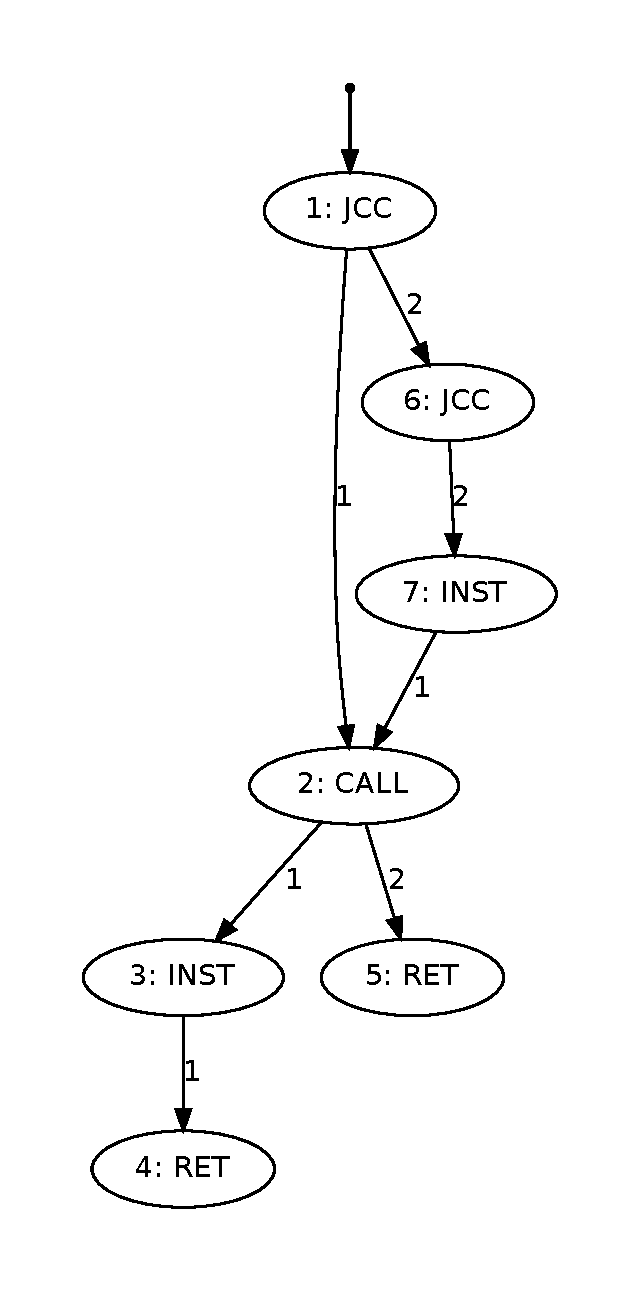
\includegraphics[height=0.4\textheight]{supports/algos/images/g1prof.pdf}
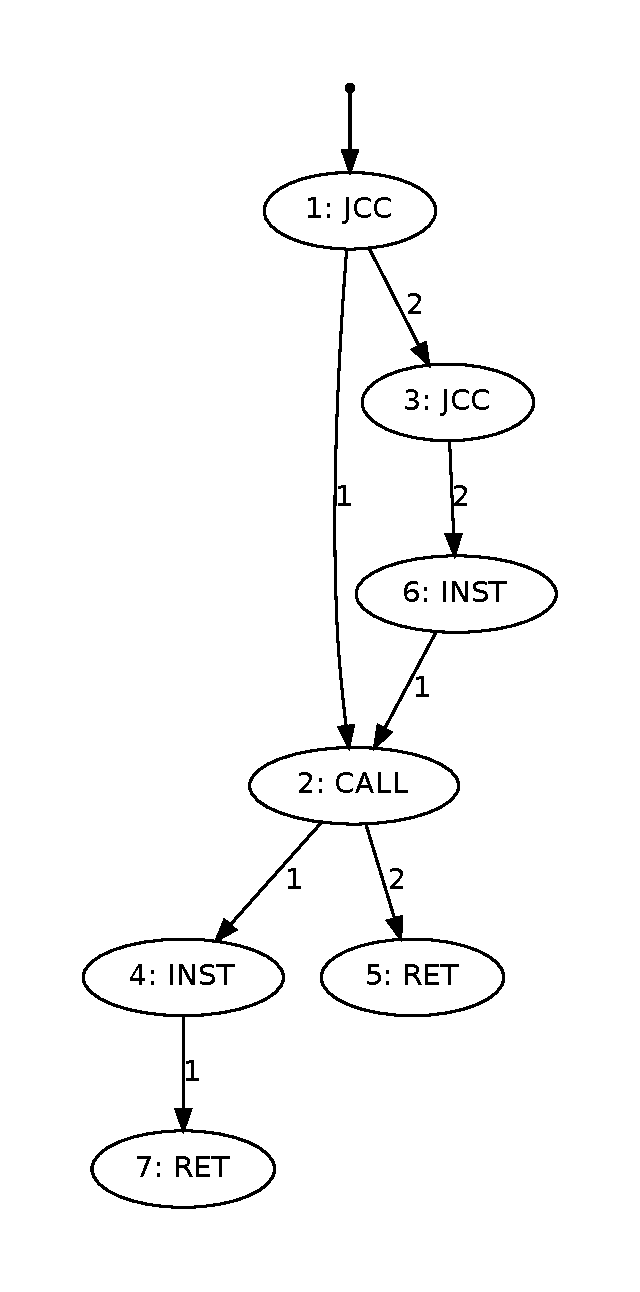
\includegraphics[height=0.4\textheight]{supports/algos/images/g1larg.pdf}
\end{center}
% \end{figure}

On peut représenter le parcours en profondeur de ce site de la manière suivante : On commence par la racine, que l'on numérote 1, c'est un JCC, puis le premier fils nous amène à un nouveau sommet, numéroté 2, c'est un CALL. Son premier fils nous amène à numéroter 3: INST et 4: RET. Une fois au $4^e$ sommet, on retourne au sommet 2 pour prendre le second fils que l'on numéroté 5: RET. On remonte au sommet 1, on numérote le second fils : c'est le sommet 6: JCC puis on prend son seul fils (fils 2) et on numéroté 7: INST. De là on prend le premier fils pour retourner sur le fils 2. Le parcours s'arrête puisqu'on a visité tous les arcs du site.\\
On peut noter le parcours ainsi (avec l'algorithme \ref{algo:codageProf}) :\\
$1: JCC\xrightarrow{1} 2: CALL \xrightarrow{1} 3: INST \xrightarrow{1} 4: RET \xrightarrow{R} 2 \xrightarrow{2} 5: RET \xrightarrow{R} 1 \xrightarrow{2} 6: JCC \xrightarrow{2} 7:INST \xrightarrow{1} 2$.\\
En fait, décrit de cette manière, le parcours définit un site unique que l'on peut reconstruire puisqu'on sait quels sont les labels de chaque sommet, tous les arcs entre les sommets et le choix des fils choisi lors du parcours (ici en profondeur).\\
De même, le parcours en largeur du site peut être décrit ainsi (avec l'algorithme \ref{algo:codageLarg}) :\\
$1: JCC\xrightarrow{1} 2: CALL\xrightarrow{R} 1\xrightarrow{2} 3: JCC\xrightarrow{R} 2\xrightarrow{1} 4: INST\xrightarrow{R} 2\xrightarrow{2} 5: RET\xrightarrow{R} 3\xrightarrow{2} 6: INST\xrightarrow{R} 4\xrightarrow{1} 7: RET$.\\
% \overset{def}



\begin{algorithm}
\caption{Codage du parcours en profondeur d'un site}
\SetAlgoLined
\KwData{Un site de racine R}
\KwResult{Le codage du parcours en profondeur de ce site}
\SetKwProg{Fn}{}{}{}
\SetKwFunction{FRecurs}{parcoursProfondeur}
\Fn(\tcc*[h]{s: sommet, i: dernier numéro attribué, E: sommets déjà explorés, etiq: associe une étiquette à un sommet, num: associe un sommet à son numéro}){\FRecurs{s, i, E, etiq, num}}{
% \Fn(// s: sommet, i: dernier numéro attribué, E: sommets déjà explorés){\FRecurs{s, i, E}}{
     \eIf{$s\notin E$}{
      $E\leftarrow E\cup\{s\}$\\
      $num(s)\leftarrow i$\\
      $C\leftarrow "i: etiq(s)"$\\
      $i\leftarrow i+1$\\
      \For{f fils numéro k de s}{
        $C\leftarrow C+"\xrightarrow{k}"$\\
	$(i, c)\leftarrow parcoursProfondeur(f, i, E, etiq, num)$\\
	$C\leftarrow C+ c$\\
	\If{s a encore au moins un fils}{
	$C\leftarrow C+ "\xrightarrow{R} num(s)"$\\
	}
      }
      	$retourner (i, C)$\\
     }
     {
     $retourner (i, "num(s)")$\\
     }
}
parcoursProfondeur(R, 1, $\emptyset$, etiq, $\emptyset$)
\label{algo:codageProf}
\end{algorithm}

\begin{algorithm}
\caption{Codage du parcours en largeur d'un site}
\SetAlgoLined
\KwData{Un site de racine R}
\KwResult{Le codage du parcours en largeur de ce site}
\SetKwProg{Fn}{}{}{}
\SetKwFunction{FRecurs}{parcoursLargeur}
\Fn(\tcc*[h]{etiq: associe une étiquette à un sommet}){\FRecurs{etiq}}{
% \Fn(// s: sommet, i: dernier numéro attribué, E: sommets déjà explorés){\FRecurs{s, i, E}}{

}
$s_c\leftarrow \epsilon$\tcc*[H]{Le sommet courant devient $\epsilon$.}
% $num(R)\leftarrow 1$\tcc*[H]{Il est numéroté 1.}
$i\leftarrow 1$\tcc*[H]{On numérote à partir de 1.}
$C\leftarrow ""$\\
$A\leftarrow [(\epsilon, 0, R)]$\tcc*[H]{A contient les sommets à visiter.}
$E\leftarrow \{\}$\tcc*[H]{E est l'ensemble des sommets déjà visités.}
\While{il y a un premier élément a=(p, k, s) dans A}{
  Retirer le premier élément de A\\
  \If{$s_c$ n'est ni p ni $\epsilon$}
  {
    $C\leftarrow C+ "\xrightarrow{R} num(p)"$\\
    $s_c\leftarrow p$
  }
  \eIf{s n'est pas dans E}
  {
    \eIf{p est $\epsilon$}{
      $C\leftarrow C+ "1: etiq(R)"$\\
    }
    {
      $C\leftarrow C+ "\xrightarrow{k} i: etiq(s)"$\\
    }
    $num(s)\leftarrow i$\\
    $i\leftarrow i+1$\\
    $s_c\leftarrow s$\\
    \For{fils f numéro k' du sommet s}
    {  
      $A\leftarrow A + (s, k', f)$
    }
    $E\leftarrow E\cup \{s\}$\\
  }
  {
    $C\leftarrow C+ "\xrightarrow{k} num(s)"$\\
    $s_c\leftarrow s$\\
  }
}
\Return C
\label{algo:codageLarg}
\end{algorithm}


On peut reconstuire le site à partir du codage précédent en procédant de manière incrémentale (algorithme \ref{algo:siteDepuisCodage}) si le codage est bien formé (définition \ref{def-codage-bien-forme}).
Par la suite on ne parlera que de codages bien formés sans l'expliciter.
\begin{defi}
\label{def-codage-bien-forme}
 Un codage de parcours est bien formé s'il vérifie :
\begin{enumerate}
 \item Il est de la forme $1:L(\xrightarrow{\alpha}i[:L])*$ avec L une étiquette et $\alpha$ un entier k ou R
 \item L'étiquette de chaque sommet est spécifiée une unique fois : lors la première référence à ce sommet
%  \item S'il y a deux mots de la forme $i:L_1$ et $i:L_2$ alors $L_1=L_2$
 \item Pour tout mot de la forme $\xrightarrow{R}i[:L]$, un mot $i:L$ est présent précédemment dans le codage
 \item Il ne définit qu'une fois chaque fils de chaque sommet : à $i$ et $k$ fixés, il ne doit y avoir qu'une seule occurence de $i[:L]\xrightarrow{k}$
%  \item Toute suite incluse dans le codage de la forme $1:L(\xrightarrow{\alpha}i[:L])*$ est également un parcours
\end{enumerate} 
\end{defi}



\begin{algorithm}[H] %or another one check
\caption{Reconstruction d'un site depuis son codage}
\SetAlgoLined
\KwData{Le codage d'un site}
\KwResult{Un site}
\SetKwProg{Fn}{}{}{}
\SetKwFunction{FRecurs}{reconstructionSite}
\Fn(\tcc*[h]{Le codage est de la forme $1:L(\xrightarrow{\alpha}i[:L])*$}){\FRecurs{codage}}{
% \Fn(// s: sommet, i: dernier numéro attribué, E: sommets déjà explorés){\FRecurs{s, i, E}}{
Création d'un site vide\\
Ajout du sommet 1 d'étiquette L qui est la racine du site et devient le sommet courant\\
  \For{chaque suite de symboles de type $\xrightarrow{\alpha}i[:L]$}{
  \eIf{$\alpha$ est un entier k}{
  Ajout du sommet i d'étiquette L s'il n'existait pas\\
  Ajout d'un arc entre le sommet courant et le sommet i\\
  Le sommet i devient le sommet courant
  }
  {
  Le sommet i devient le sommet courant
  }
  }
}
\label{algo:siteDepuisCodage}
\end{algorithm}
% \begin{prop}
% Soit $S_1$ et $S_2$ deux sites dont les codages de parcours en profondeur (générés par l'algorithme \ref{algo:codageProf}) sont $C_1$ et $C_2$.\\
% $C_1=C_2\Rightarrow S_1$ et $S_2$ sont deux sites isomorphes.
% \end{prop}
% 
% \begin{pr}
%  On a supposé que l'algorithme \ref{algo:siteDepuisCodage} inverse l'algorithme \ref{algo:codageProf} pour des codages bien formés.
% \end{pr}
% 
% \begin{prop}
% \label{prop:isoCodage}
% Soit $C_1$ et $C_2$ deux codages de parcours dont les sites résultants (par l'algorithme \ref{algo:siteDepuisCodage}) sont $S_1$ et $S_2$.\\
% $S_1$ et $S_2$ sont deux sites isomorphes $\Rightarrow C_1=C_2$.\\
% (c'est faux)
% \end{prop}
% 
L'algorithme \ref{algo:parcoursSiteDepuisCodage} tente de trouver le sous-site désigné par un codage dans un graphe de flot T, à partir d'un sommet donné. S'il ne renvoie pas FAIL, il fournit un site qui est effectivement un sous-site du graphe (les sommets et les arcs sont forcément dans T, et ils sont accessibles à partir de la racine vu qu'il s'agit d'un parcours).

\begin{algorithm}[H] %or another one check
\caption{Reconstruction d'un sous-site de graphe de flot à partir d'un sommet donné, depuis son codage}
\SetAlgoLined
\KwData{Le codage d'un site, un graphe de flot T, un sommet R de T}
\KwResult{Un site ou FAIL}
\SetKwProg{Fn}{}{}{}
\SetKwFunction{FRecurs}{reconstructionSousSite}
\Fn(\tcp*[h]{Le codage est de la forme $1:L(\xrightarrow{\alpha}i[:L])*$}){\FRecurs{codage, T, R}}{
\eIf{le sommet R a l'étiquette L}{
  On numérote R par 1.\\
  Le sommet numéroté 1 devient le sommet courant.
}
{
  \Return FAIL
}
  \For{chaque suite de symboles de type $\xrightarrow{\alpha}i[:L]$}{
  \eIf{$\alpha$ est un entier k}{
  \uIf{le sommet courant a un fils k non numéroté, d'étiquette L, et aucun sommet n'est numéroté i}{
  On numérote ce fils k par i.\\
  Le sommet numéroté i devient le sommet courant.
  }
  \uElseIf{le sommet courant a un fils k numéroté i}{
  Le sommet numéroté i devient le sommet courant.
  }
  \Else{
  \tcp{Le parcours n'est pas possible si :\\ un autre sommet est déjà numéroté i,  ou\\ si le sommet à numéroter a déjà une autre numérotation,  ou\\ si l'étiquette n'est pas la bonne, ou\\ s'il n'y a pas de fils k}
  \Return FAIL
  }
  }
  {
  Le sommet i devient le sommet courant
  }
  }
  \Return le site constitué des sommets numérotés et des arcs empruntés.
}
\label{algo:parcoursSiteDepuisCodage}
\end{algorithm}

On voudrait maintenant prouver l'équivalence entre l'existence d'un isomorphisme de sous-site entre un site P et un graphe de flot T d'une part, et la possibilité d'appliquer un parcours bien formé quelconque de P à partir d'un sommet de T. Les deux propositions suivantes vont permettre d'établir l'équivalence statuée au théorème \ref{theo:eqIsoCodage}.

\begin{prop}
 Soit un codage C d'un parcours, $S_C$ son site associé par l'algorithme \ref{algo:siteDepuisCodage}, T un graphe de flot et R un sommet de T.\\
 Si un parcours de T à partir de R renvoie un site S (algorithme \ref{algo:parcoursSiteDepuisCodage}), alors $S_C$ et S sont isomorphes.
 \label{prop:condageDoncIso}
\end{prop}

\begin{pr}
 Les sous-sites restreints à leur racine sont isomorphes (un seul sommet avec la même étiquette), numérotés de la même manière et le sommet courant est le même.\\
 Supposons que les sous sites restreints aux sommets du parcours $1:L_1\xrightarrow{\alpha_1}i_2[:L_2]\xrightarrow{\alpha_2} ...\xrightarrow{\alpha_{p-1}}i_{p}[:L_{p}]$ sont isomorphes.\\
 Lors de l'étape suivante du parcours ($\xrightarrow{\alpha}i[:L]$), le seul cas où un sommet est numéroté est si $\alpha$ est un entier $k$, si le sommet courant dans T a un fils k non numéroté d'étiquette L et aucun sommet n'est déjà numéroté i. Dans cas un sommet est ajouté au site créé par l'algorithme \ref{algo:siteDepuisCodage} à partir du sommet courant. Dans les deux cas la numérotation est la même et le sommet courant est le sommet qui vient d'être numéroté ou ajouté.\\
 Le second cas possible est si le sommet courant a un fils k déjà numéroté i et d'étiquette L. Dans ce cas ce sommet a déjà été ajouté au sité créé par l'algorithme \ref{algo:siteDepuisCodage}, il n'y a ni numérotation ni ajout de site et le sommet courant devient le fils k.\\
  Les arcs sont nécessairement les mêmes puisque les parcours appliqués dans les deux algorithmes sont identiques. \\
 Tous les autres cas provoquent un arrêt du parcours par un FAIL. \\
 On a bien montré que dans les cas ne provoquant pas d'erreur, les deux sites restreints aux sommets du parcours sont isomorphes.
\end{pr}

\begin{prop}
 Si P est un site isomorphe à un sous-site S d'un graphe de flot T alors tout codage de parcours $C_P$ de P peut être parcouru dans T à partir de la racine de S.
 \label{prop:isoDoncCodage}
\end{prop}

\begin{pr}
On va montrer que l'algorithme \ref{algo:parcoursSiteDepuisCodage} appliqué au codage $C_P$, au graphe T, à partir de la racine de S produit un site S' isomorphe à S et P. \\
Le graphe composé uniquement de la racine de P est isomorphe à celui composé de la racine de S ajoutée au graphe à construire dans l'algorithme \ref{algo:parcoursSiteDepuisCodage}. \\
Supposons que les sous sites restreints aux sommets du parcours $1:L_1\xrightarrow{\alpha_1}i_2[:L_2]\xrightarrow{\alpha_2} ...\xrightarrow{\alpha_{p-1}}i_{p}[:L_{p}]$ sont isomorphes et que les numérotations correspondent à l'isomorphisme.\\
Lors de l'étape suivante du parcours ($\xrightarrow{\alpha}i[:L]$), un sommet n'est ajouté dans l'algorithme \ref{algo:siteDepuisCodage} que si $\alpha$ est un entier $k$ et si le sommet $i$ n'a pas déjà été créé. Dans le parcours de T (algorithme \ref{algo:parcoursSiteDepuisCodage}), cela implique qu'aucun sommet n'est déjà numéroté $i$. Puisque le sommet courant dans P a un fils $k$, que les sommets courants de P et S' sont correspondant dans l'isomorphisme et que P et S sont isomorphes, le sommet courant dans S' a un fils $k$ (d'étiquette $L$). Puisque le codage est bien formé, il n'y a qu'un fils $k$ du sommet courant. Ce fils $k$ n'a pas déjà été numéroté, sinon il aurait déjà été créé précédemment dans l'algorithme \ref{algo:siteDepuisCodage}. On est donc nécessairement dans le cas où on numérote le fils $k$ du sommet courant par i, le sommet ajouté dans l'algorithme \ref{algo:siteDepuisCodage} porte le même numéro que celui numéroté dans le parcours de T : ils se correspondent dans un isomorphisme de 
sites.\\
Dans le cas contraire où aucun fils n'est ajouté, comme précédemment le sommet courant a nécessairement un fils $k$ qui a déjà été numéroté puisque c'est le cas dans la reconstruction du site P. Dans les deux cas aucun site n'est ajouté mais le fils $k$ devient le sommet courant.\\
On en déduit que les sommets ajoutés sont toujours deux sommets correspondants dans un isomorphisme et que les arcs ajoutés sont également les mêmes.
\end{pr}

\begin{theo}
 Soit P un site et T un graphe de flot. Les deux propositions suivantes sont équivalents :
 \begin{itemize}
  \item P est isomorphe à un sous-site de T
  \item Il existe C un codage de parcours bien formé de P tel que le parcours de C est possible dans T
 \end{itemize}
\label{theo:eqIsoCodage}
\end{theo}

\begin{pr}
~
 \begin{itemize}
 \renewcommand{\labelitemi}{$\bullet$}
  \item Si P est isomorphe à un sous-site de T, on peut appliquer la proposition \ref{prop:isoDoncCodage} au parcours en profondeur, ce qui donne directement le résultat.
  \item S'il existe un codage C de parcours de P que l'on peut également parcourir dans T, alors on construit son site associé avec l'algorithme \ref{algo:siteDepuisCodage} et on applique la proposition \ref{prop:condageDoncIso} qui donne le résultat.
 \end{itemize}
\end{pr}

L'intérêt de cet équivalence est qu'elle donne un algorithme simple et bien plus efficace que celui d'Ullmann pour résoudre le problème \ref{pbisosg} d'isomorphisme de sous-site entre un site de motif et un graphe de flot de test.

\subsection{Application directe}
\subsubsection{Résolution des problèmes d'isomorphisme}
L'équivalence entre isomorphisme et parcours permet de résoudre le problème \ref{pbisog} de la manière suivante :
Deux sites sont isomorphes si et seulement si leurs codages de parcours en profondeur\footnote{On peut substituer le parcours en profondeur par un parcours en largeur on n'importe quel codage de parcours bien formé} sont identiques.

Le problème \ref{pbisosg} de l'existence d'un isomorphisme entre un site et un sous-site d'un site peut être résolu ainsi :
Il existe un sous-site de T isomorphe au site P si et seulement si il existe un sommet de T à partir duquel le codage du parcours en profondeur\footnotemark[\value{footnote}] de P est possible.

Une solution au problème \ref{pbisosgbase} de l'existence d'un site dans une base $L_S$ isomorphe à un sous-site d'un site T consiste à itérer la solution précédente de l'isomorphisme de sous-site à chaque site de la base $L_S$.

\subsubsection{Complexité}
La résolution du problème de l'isomorphisme de sous-site avec cet algorithme se réalise dans le pire des cas en $O(n_T.n_P)$ puisqu'elle nécessite :
\begin{itemize}
 \item Un parcours en profondeur du site de motif P avec détermination du codage : $O(n_P)$
 \item Un parcours du graphe de flot T à partir de chacun de ses sommets : chaque parcours se fait en $O(n_P)$, cette étape peut alors se réaliser en $O(n_T.n_P)$
\end{itemize}
~\\

Si on a une base de $n$ sites $L_S$ de taille $W$, la complexité dans le pire des cas pour déterminer un site de la base est isomorphe à un sous-site de T est $O(n.n_T.W)$.


\subsection{Codages rangés dans un arbre de décision}
\subsubsection{Création d'un arbre de décision des codages}
On peut générer les codages de parcours en profondeur de chaque site de la base puis les ranger dans un arbre de décision. Par exemple trois sites donnés en figure \ref{fig:troisProf}, dont les parcours en profondeur sont (dans l'ordre):\\
$1: JCC\xrightarrow{1} 2: CALL \xrightarrow{1} 3: INST \xrightarrow{1} 4: RET \xrightarrow{R} 2 \xrightarrow{2} 5: RET \xrightarrow{R} 1 \xrightarrow{2} 6: JCC \xrightarrow{2} 7:INST \xrightarrow{1} 2$
\\
$1: JCC\xrightarrow{1} 2: CALL \xrightarrow{1} 3: INST \xrightarrow{1} 4: RET \xrightarrow{R} 2 \xrightarrow{2} 5: RET \xrightarrow{R} 1 \xrightarrow{2} 6: JCC \xrightarrow{2} 7:INST \xrightarrow{1} 3$
\\
$1: JCC\xrightarrow{1} 2: RET \xrightarrow{R} 1 \xrightarrow{2} 3: JCC \xrightarrow{2} 4: INST \xrightarrow{1} 5: CALL \xrightarrow{1} 6: INST \xrightarrow{1} 2 \xrightarrow{R} 5 \xrightarrow{2} 7: RET$

L'arbre de décision créé à partir de ces trois codages est donné en figure \ref{fig:arbreDecTarjan}. L'ajout d'un codage à l'arbre de décision est standard et ne sera pas détaillée.

\begin{figure}
\begin{center}
\subfigure[]{
\label{fig:troisProf1}
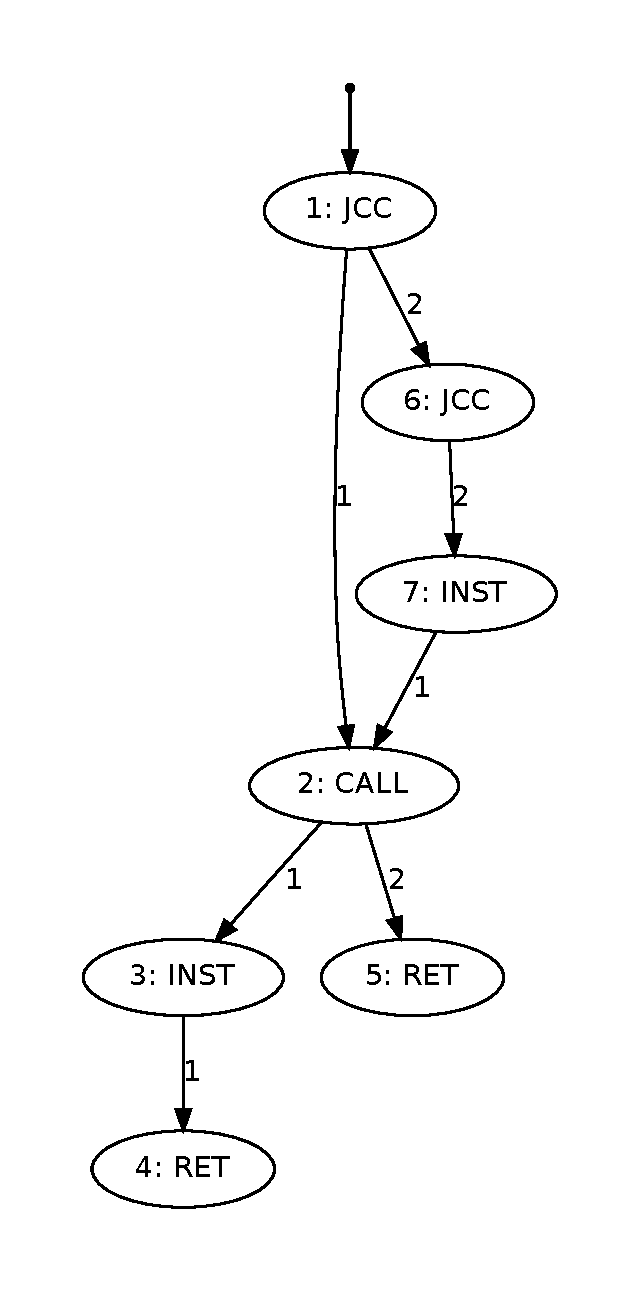
\includegraphics[height=0.4\textheight]{supports/algos/images/g1prof.pdf}}
\subfigure[]{
\label{fig:troisProf2}
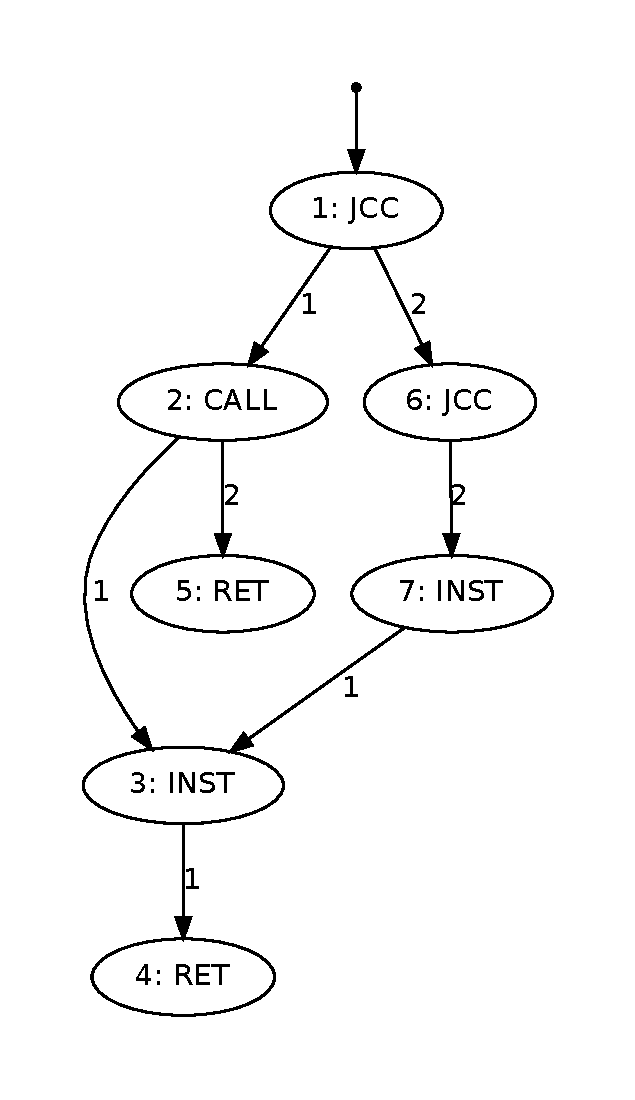
\includegraphics[height=0.4\textheight]{supports/algos/images/g2prof.pdf}}
\subfigure[]{
\label{fig:troisProf3}
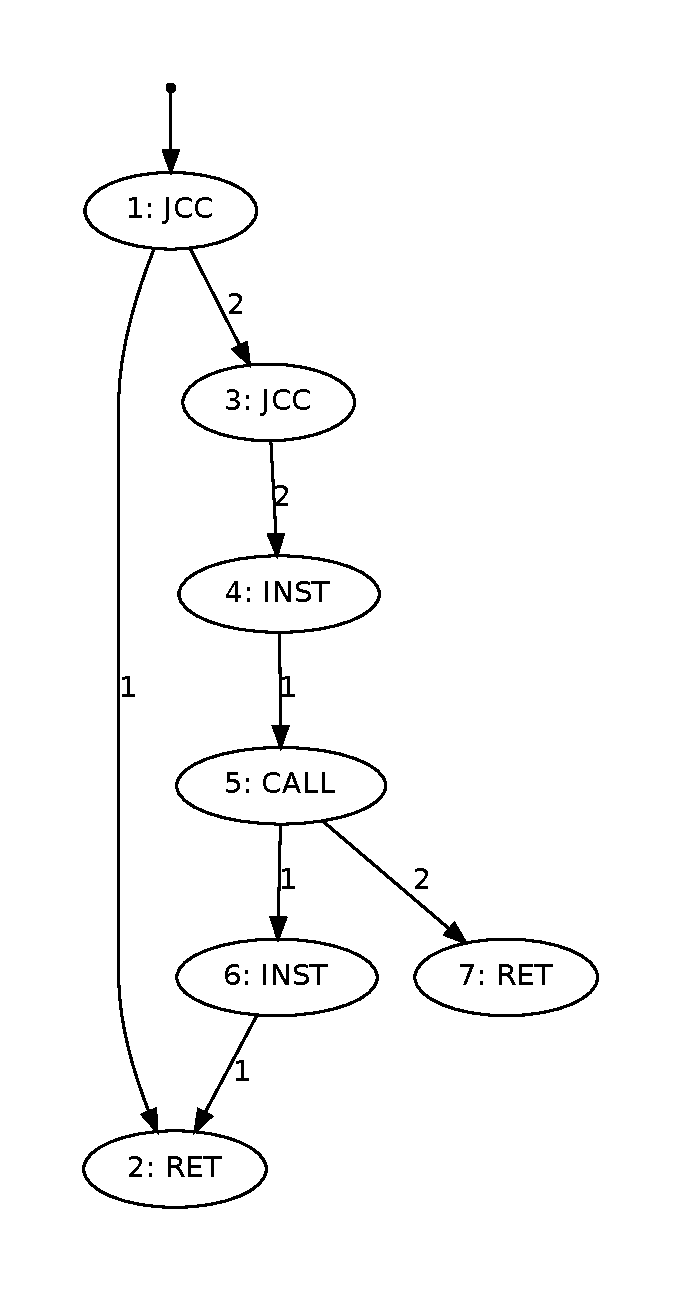
\includegraphics[height=0.4\textheight]{supports/algos/images/g3prof.pdf}}
\end{center}
\caption{Trois sites numérotés selon un parcours en profondeur}
\label{fig:troisProf}
\end{figure}
% $1: JCC\xrightarrow{1} 2: CALL \xrightarrow{1} 3: INST \xrightarrow{1} 4: RET \xrightarrow{R} 2 \xrightarrow{2} 5: RET \xrightarrow{R} 1 \xrightarrow{2} 6: JCC \xrightarrow{2} 7:INST \xrightarrow{1} 2$

\begin{figure}
\begin{center}
\begin{tikzpicture}[
  tlabel/.style={pos=0.4,right=-1pt,font=\footnotesize\color{black!70!black} },
  every node/.style={color=black!25!black, circle, minimum size=6mm, draw=black!75, align=center},
  edge from parent/.style={draw=black!50,thick},
  level 1/.style={sibling distance=50mm, level distance=12mm},
]
\node[rectangle, rounded corners]{$racine$}
child {node {}
       child{node {}
	     child {node {}
	            child {node {}
		           child {node {}
		                  child {node {}
		                         child {node {}
		                                child {node {}
		                                       child {node {}
		                                              child {node {a}
								edge from parent node[tlabel,pos=0.2, left=15pt,draw=none] {$\xrightarrow{1} 2$}
		                                              }
		                                              child {node {b}
								edge from parent node[tlabel,pos=0.2, right=11pt,draw=none] {$\xrightarrow{1} 3$}
		                                              }
		                                              edge from parent node[tlabel,pos=0.3,draw=none] {$\xrightarrow{2} 7:INST$}
		                                       }
		                                       edge from parent node[tlabel,pos=0.3,draw=none] {$\xrightarrow{2} 6: JCC$}
		                                }
		                                edge from parent node[tlabel,pos=0.3,draw=none] {$\xrightarrow{R} 1$}
		                         }
		                         edge from parent node[tlabel,pos=0.3,draw=none] {$\xrightarrow{2} 5: RET$}
		                  }
		                  edge from parent node[tlabel,pos=0.3,draw=none] {$\xrightarrow{R} 2$}
		           }
		           edge from parent node[tlabel,pos=0.3,draw=none] {$\xrightarrow{1} 4: RET$}
	            }
	            edge from parent node[tlabel,pos=0.3,draw=none] {$\xrightarrow{1} 3: INST$}
	     }
	     edge from parent node[tlabel,pos=0.1, left=15pt,draw=none] {$\xrightarrow{1} 2: CALL$}
       }
       child{node {}
	     child {node {}
	            child {node {}
		           child {node {}
		                  child {node {}
		                         child {node {}
		                                child {node {}
		                                       child {node {}
		                                              child {node {c}
		                                              edge from parent node[tlabel,pos=0.3,draw=none] {$\xrightarrow{2} 7: RET$}
		                                              }
		                                              edge from parent node[tlabel,pos=0.3,draw=none] {$\xrightarrow{R} 5$}
		                                       }
		                                       edge from parent node[tlabel,pos=0.3,draw=none] {$\xrightarrow{1} 2$}
		                                }
		                                edge from parent node[tlabel,pos=0.3,draw=none] {$\xrightarrow{1} 6: INST$}
		                         }
		                         edge from parent node[tlabel,pos=0.3,draw=none] {$\xrightarrow{1} 5: CALL$}
		                  }
		                  edge from parent node[tlabel,pos=0.3,draw=none] {$\xrightarrow{2} 4: INST$}
		           }
		           edge from parent node[tlabel,pos=0.3,draw=none] {$\xrightarrow{2} 3: JCC$}
	            }
	            edge from parent node[tlabel,pos=0.3,draw=none] {$\xrightarrow{R} 1$}
	     }
	     edge from parent node[tlabel,pos=0.1, right=5pt,draw=none] {$~~~\xrightarrow{1} 2: RET$}
       }
       edge from parent node[tlabel,pos=0.5,draw=none] {$1: JCC$}
};
\end{tikzpicture}
\end{center}
\caption{Arbre de décision contenant les codages de sites de la figure \ref{fig:troisProf}}
\label{fig:arbreDecTarjan}
\end{figure}

\paragraph{Complexité.}
L'ajout d'un site à la base consiste à ajouter un codage de parcours dans l'arbre de décision, cette opération nécessite un nombre de comparaison en $W.i$ où $i$ est le nombre de fils maximum de chaque sommet de l'arbre. Vue que les étiquettes des arcs de l'arbre sont de la forme $[\xrightarrow{\alpha}]i[:L]$, en notant $K$ le nombre de fils maximum de chaque sommet dans un site et $n_L$ le nombre d'étiquettes différentes pour les sommets des sites, $i\leq (K+2).W.n_L$ soit $n=O(W)$ donc l'ajout d'un site à la base se fait en $O(W^2)$.

\subsubsection{Recherche d'un isomorphisme de sous-sites à partir de l'arbre de décision}
Une fois l'arbre généré à partir de tous les codages des sites de $L_S$, on veut l'utiliser pour trouver tous les parcours de $L_S$ possibles dans le graphe de flot T. Pour compter le nombre de parcours de l'arbre que l'on peut réaliser à partir du sommet $r$ de $T$, on peut chercher à parcourir $T$ à partir de $r$ en parcourant les branches possibles dans l'arbre de décision. À chaque fois qu'on peut parcourir une branche jusqu'en bas c'est qu'un site isomorphe a été trouvé. L'algorithme \ref{algo:rechercheArbreTarjan} compte le nombre de ces branches possibles.

On peut utiliser cet algorithme pour retrouver tous les sous-sites isomorphes en utilisant l'algorithme précédent à partir de chaque sommet de $T$.

\begin{figure}
\begin{algorithm}[H] %or another one check
\caption{Décompte des parcours d'un arbre de parcours possibles dans un graphe de flot, à partir d'un sommet donné}
\SetAlgoLined
\KwData{Un arbre A contenant les parcours de sites, un graphe de flot T, un sommet r de T}
\KwResult{Le nombre de parcours possibles}
\SetKwProg{Fn}{}{}{}
\SetKwFunction{FRecurs}{decompteSousSite}
\Return decompteSousSite(A, racine(A), T, r)\\
~\\

\Fn{\FRecurs{A, a, T, R}}{
  \eIf{a n'a aucun fils dans A}{
    \tcp{Si a n'a aucun fils, on a exactement décrit un parcours}
    \Return 1
  }
  {
    $somme\leftarrow 0$\\
    \For{f fils d'étiquette e de a dans A}{
	$(possible, s', T') \leftarrow etape(e, s, T)$\\
	\If{possible}{
	  $somme\leftarrow somme+decompteSousSite(A, f, T', s')$
	}
    }
  }
}

\SetKwProg{Fn}{}{}{}
\SetKwFunction{FRecurs}{etape}
\Fn(\tcp*[h]{L'étiquette e est de la forme $[\xrightarrow{\alpha}]i[:L]$}){\FRecurs{e, s, T}}{
  \eIf{e est de la forme $1:L$}{
    Numéroter le sommet s de T par 1.\\
    \Return (true, s, T)
  }
  {
    \tcp{Dans ce cas e est de la forme $\xrightarrow{\alpha}i[:L]$}
    \eIf{$\alpha$ est un entier k}{
    \uIf{s a un fils s' d'ordre k non numéroté dans T, d'étiquette L, et aucun sommet n'est numéroté i}{
    On numérote s' par i dans T.\\
    \Return $(true, s', T)$
    }
    \uElseIf{le sommet courant a un fils s' d'ordre k numéroté i}{
    \Return $(true, s', T)$
    }
    \Else{
    \tcp{Le parcours n'est pas possible si :\\ un autre sommet est déjà numéroté i,  ou\\ si le sommet à numéroter a déjà une autre numérotation,  ou\\ si l'étiquette n'est pas la bonne, ou\\ s'il n'y a pas de fils k}
    \Return $(false, s ,T)$
    }
    }
    {
      \tcp{Dans ce cas e est de la forme $\xrightarrow{R}i$}
      On note s' le sommet numéroté i dans T.\\
      \Return $(true, s', T)$
    }
  }
}
\label{algo:rechercheArbreTarjan}
\end{algorithm}
\end{figure}

\paragraph{Complexité.}
Dans le pire des cas il y a $n$ branches à l'arbre A qui partent de la racine où $n$ est le nombre de sites dans la base. Le parcours d'une branche avec au maximum un fils à chaque sommet, à partir de la racine se fait en $O(W)$ au vu de la récursion de l'algorithme  \ref{algo:rechercheArbreTarjan}. Pour chercher les isomorphismes de sous-sites de $T$ il faut répéter l'opération pour chacun de ses sommets : la complexité totale dans le pire des cas pour résoudre le problème \ref{pbisosgbase} d'isomorphisme de sous-sites entre un graphe de flot et une base de sites est de $O(n.n_T.W)$. Ainsi on n'a pas amélioré la complexité dans le pire des cas par rapport à l'utilisation directe du parcours de Tarjan vu dans la section précédente, bien qu'en pratique l'algorithme soit plus rapide comme nous le verrons par la suite.

\clearpage
\section{SIDT : Site Isomorphism Decision Tree}
Le problème \ref{pbisosg} consiste à détecter un site P dans un graphe de flot T. En pratique le site P aura été généré à partir d'un graphe de flot G. Si P est un sous-site de T, puisqu'on a généré le site à partir d'un parcours dans un autre graphe de flot, on peut envisager que le même parcours appliqué à T est susceptible de générer le site P. Ce n'est pas vrai dans le cas général et en ce sens l'algorithme présenté ici n'est pas complet.\\
Inversement il est clair que si le même parcours appliqué à partir de sommets de T et G génèrent le même site P, alors P est bien un sous-site de T.
\\

On se propose donc, pour approcher la solution au problème \ref{pbisosg} de détection d'isomorphisme de sous-site entre un site P (généré par parcours avec un algorithme A à partir d'un sommet d'un graphe de flot G) et un graphe de flot T, de générer tous les sous-sites de T avec l'algorithme de parcours A et de regarder si P est dans cet ensemble.

Pour régler le problème \ref{pbisosgbase} de détection d'un site dans une base de graphes de flot, on va créer un arbre de décision contenant tous les sites générés à partir du parcours par A des graphes de flot de la base.

\subsection{Arbre de décision pour la détection de sites}
Chaque site est généré par un parcours numérotant ses sommets, et chaque sommet a un nombre de fils bornés. On représente alors les sites sous forme matricielle : chaque ligne représente un sommet, le premier élément de la colonne est l'étiquette du sommet et les éléments suivants sont les numéros des fils de ce sommet (0 indique qu'il n'y a pas de sommet). La représentation des sites de la figure \ref{fig:troisProf} est donnée figure \ref{fig:troisProfMatRed}.
On peut ensuite agréger tous les sites générés dans un arbre de décision (figure \ref{fig:arbreDecTarjan}).

\begin{figure}
\begin{center}
\subfigure[]{
\label{fig:troisProfMatRed1}
$\begin{array}{r|ccc} Sommet & Etiquette & Fils 1 & Fils 2 \\
\hline
1 & JCC & 2 & 6\\
2 & CALL & 3 & 5\\
3 & INST & 4 & 0\\ 
4 & RET & 0 & 0\\ 
5 & RET & 0 & 0\\ 
6 & JCC & 0 & 7\\ 
7 & INST & 2 & 0\\ 
\end{array}$
}
\subfigure[]{
\label{fig:troisProfMatRed2}
$\begin{array}{r|ccc} Sommet & Etiquette & Fils 1 & Fils 2 \\
\hline
1 & JCC & 2 & 6\\
2 & CALL & 3 & 5\\
3 & INST & 4 & 0\\ 
4 & RET & 0 & 0\\ 
5 & RET & 0 & 0\\ 
6 & JCC & 0 & 7\\ 
7 & INST & 3 & 0\\ 
\end{array}$
}
\subfigure[]{
\label{fig:troisProfMatRed3}
$\begin{array}{r|ccc} Sommet & Etiquette & Fils 1 & Fils 2 \\
\hline
1 & JCC & 2 & 3\\
2 & RET & 0 & 0\\
3 & JCC & 0 & 4\\ 
4 & INST & 5 & 0\\ 
5 & CALL & 6 & 7\\ 
6 & INST & 2 & 0\\ 
7 & RET & 0 & 0\\ 
\end{array}$
}
\end{center}
\caption{Représentation matricielle des sites de la figure \ref{fig:troisProf}}
\label{fig:troisProfMatRed}
\end{figure}

\begin{figure}
\begin{center}
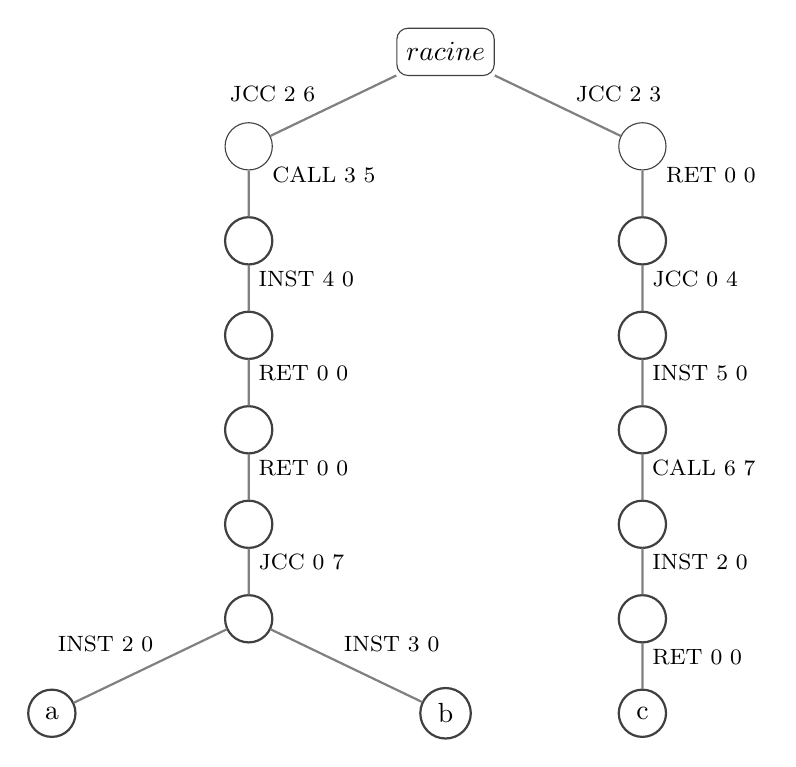
\begin{tikzpicture}[
  tlabel/.style={pos=0.4,right=-1pt,font=\footnotesize\color{black!70!black} },
  every node/.style={color=black!25!black, circle, minimum size=6mm, draw=black!75, align=center},
  edge from parent/.style={draw=black!50,thick},
  level 1/.style={sibling distance=50mm, level distance=12mm},
]
\node[rectangle, rounded corners]{$racine$}
child{node{}
      child{node {}
	     child {node {}
	            child {node {}
		           child {node {}
		                  child {node {}
		                         child {node {a}
		                                edge from parent node[tlabel,pos=0.2, left=10pt,draw=none] {INST 2 0}
		                         }
		                         child {node {b}
		                                edge from parent node[tlabel,pos=0.2, right=12pt,draw=none] {INST 3 0}
		                         }
		                         edge from parent node[tlabel,pos=0.3,draw=none] {JCC 0 7}
		                  }
		                  edge from parent node[tlabel,pos=0.3,draw=none] {RET 0 0}
		           }
		           edge from parent node[tlabel,pos=0.3,draw=none] {RET 0 0}
	            }
	            edge from parent node[tlabel,pos=0.3,draw=none] {INST 4 0}
	     }
	     edge from parent node[tlabel,pos=0.1, right=5pt,draw=none] {CALL 3 5}
       }
       edge from parent node[tlabel,pos=0.3,left=10pt,draw=none] {JCC 2 6}
      }
child {node {}
       child{node {}
	     child {node {}
	            child {node {}
		           child {node {}
		                  child {node {}
		                         child {node {c}
		                                edge from parent node[tlabel,pos=0.3,draw=none] {RET 0 0}
		                         }
		                         edge from parent node[tlabel,pos=0.3,draw=none] {INST 2 0}
		                  }
		                  edge from parent node[tlabel,pos=0.3,draw=none] {CALL 6 7}
		           }
		           edge from parent node[tlabel,pos=0.3,draw=none] {INST 5 0}
	            }
	            edge from parent node[tlabel,pos=0.3,draw=none] {JCC 0 4}
	     }
	     edge from parent node[tlabel,pos=0.1, right=5pt,draw=none] {RET 0 0}
       }
       edge from parent node[tlabel,pos=0.3,right=12pt,draw=none] {JCC 2 3}
};
\end{tikzpicture}
\end{center}
\caption{Arbre de décision contenant les matrices de la figure \ref{fig:troisProfMatRed}}
\label{fig:arbreDecSIDT}
\end{figure}

\paragraph{Complexité.}
L'apprentissage d'un site nécessite le parcours d'au plus W éléments de l'arbre de décision. Chaque sommet de l'arbre de décision a au plus $n_L.W.W$ fils où $n_L$ est le nombre d'étiquettes possibles. L'apprentissage d'un site se fait donc en $O(W^3)$ où W est le nombre de sommets des sites à apprendre.

\subsection{Recherche d'un isomorphismes de sous-sites}
Rechercher un isomorphisme de sous-sites à partir de l'arbre de décision ainsi créé revient à écrire le site sous forme matricielle et à faire une recherche dans l'arbre de décision.

\paragraph{Complexité.}
La complexité de la recherche d'un site dans l'arbre de décision est la même que pour l'ajout dans d'un site dans l'arbre et se fait en $O(W^3)$. 


\section{Comparaisons des performances}
On a donc trois algorithmes à comparer : l'algorithme d'Ullmann, pris pour référence, l'algorithme de Tarjan avec arbre de décision et l'algorithme incomplet par arbre de décision (SIDT).

\begin{center}
\begin{tabular}{|c|c|c|}
 \hline
 Algorithme & Ajout d'un site dans la base & Détection d'un site\\
 \hline
 Ullmann & (pas de base) & $O(n.(n_T.P)^{n_P})$ \\
 Tarjan avec arbre de décision & $O(W^2)$ & $O(n.n_T.W)$\\
 SIDT & $O(W^3)$ & $O(W^3)$\\
 \hline
\end{tabular} 
\end{center}

Du point de vue la complexité dans le pire des cas, il est clair que l'algorithme d'Ullmann est très inefficace et l'algorithme SIDT devrait s'avérer être le plus rapide avec une complexité constante lors de l'agrandissement de la base.


